\documentclass[11pt]{article}
\usepackage{geometry}
\usepackage{graphicx}
\usepackage{times}
\usepackage{setspace}
\usepackage[hidelinks]{hyperref}
\usepackage{tocloft}
\usepackage{caption}
\usepackage{pdflscape}
\usepackage{fancyhdr}
\usepackage{lastpage}
\usepackage{array}
\usepackage{booktabs}
\usepackage{float}
\usepackage{tabularx}
\geometry{a4paper, margin=1in}

\makeatletter
% Adjust spacing in the Table of Contents
% \renewcommand{\numberline}[1]{#1\hspace{1em}} % Adjust 1em for space after the number

% Adjust spacing in the List of Figures
\renewcommand{\l@figure}{\@dottedtocline{1}{1.5em}{3em}} % Adjust the 3em for spacing after figure number

% Adjust spacing in the List of Tables
\renewcommand{\l@table}{\@dottedtocline{1}{1.5em}{3em}} % Adjust the 3em for spacing after table number
\makeatother

\renewcommand{\cftsecleader}{\cftdotfill{\cftdotsep}}
\renewcommand{\headrulewidth}{0pt}

\newcommand{\Table}[2]{
  \begin{table}[H]
    \captionsetup{justification=raggedright, singlelinecheck=false}
    \caption{\textit{#1}}
    \renewcommand{\arraystretch}{1.5}
    \setlength{\tabcolsep}{4pt}
    \begin{tabular}{|*{100}{c|}}
      \hline
      #2 \\
      \hline
    \end{tabular}
  \end{table}
}

\newcommand{\TableWide}[2]{
  \begin{table}[H]
    \captionsetup{justification=raggedright, singlelinecheck=false}
    \caption{\textit{#1}}
    \renewcommand{\arraystretch}{1.5}
    \setlength{\tabcolsep}{4pt}
    \resizebox{\textwidth}{!}{
      \begin{tabular}{|*{100}{c|}}
        \hline
        #2 \\
        \hline
      \end{tabular}
    }
  \end{table}
}

\counterwithin{figure}{section}
\counterwithin{table}{section}

\pagestyle{fancy}
\fancyhf{}
\fancyhead{}
\fancyfoot[C]{Page \textbf{\thepage} of \textbf{\pageref{LastPage}}}

\fancypagestyle{plain}{
    \fancyhf{}
    \fancyfoot[C]{Page \textbf{\thepage} of \textbf{\pageref{LastPage}}}
}

\begin{document}

\onehalfspacing

\begin{center}
  
\includegraphics[width=0.6\textwidth]{images/AUB-MSFEA.png} \\[1cm]
  
  \LARGE \textbf{American University of Beirut} \\
  \Large School of Engineering and Architecture \\
  \Large Department of Electrical and Computer Engineering \\
  \huge \textbf{A Database Design for NexStore Company} \\[1cm]
  
  
\includegraphics[width=0.5\textwidth]{images/logo.png} \\[1cm]
  
  \Large \textbf{By} \\
  \large Jad Shaker (Group Leader) \\
  \texttt{jss31@mail.aub.edu} \\
  Hamza Atout \\
  \texttt{hsa60@mail.aub.edu} \\
  Khaled Ammoura \\
  \texttt{kaa74@mail.aub.edu} \\[1cm]
  
  \Large \textbf{A REPORT} \\
  submitted to Dr. Hussein Bakri in partial fulfillment of the requirements of phase 2 of the database project \\
  for the course \textbf{EECE433 -- Database Systems} \\[1cm]
  
  \large October 2024
\end{center}

\newpage

\tableofcontents

\phantomsection
\addcontentsline{toc}{section}{List of Figures}
\listoffigures

\phantomsection
\addcontentsline{toc}{section}{List of Tables}
\listoftables

\newpage

\section{Introduction}

"Data is the new oil, and databases are the engines that refine it". In today's competitive retail world, firms must manage both their physical and online operations efficiently to fulfill customer expectations and maximize resources. The design of a full database is important to ease the integration of inventory, sales, and customer information, and provide connection operations between both channels. This report portrays the architecture of a database for a retail business that operates in both physical and online modes, represented through an Entity-Relationship (ER) diagram.

The main goal of this database is to offer flawless coordination across the store's physical inventory and its online site. The ER diagram highlights the connection between significant entities such as Customers, Products, Orders, and Employees demonstrating how data interacts within the system. It acts as the core of the database that maintains efficient retail processes, ensuring correctness, consistency, and scalability.

This report represents NexStore company's main database design using an Entity-Relationship diagram. The References section contains all the used citations. The Tools section describes all the instruments used to draw database design. The System Description and Requirements section defines all the needs of the client. The Legend of ER diagram symbols include all the symbols of the used notation. The complete ER diagram is presented in the ER diagram for the NexStore database section. In the subsection "Entity Types \& Their Attributes", we elucidate the various types and attributes of each entity. In the other subsection "Relationships and Their Explanations", all relationships are listed and explained. In the "Conclusion" section, we summarize the main points of the design document.

\section{References / Copyright Section}

\begin{thebibliography}{9}
  \bibitem{elmasri}
  \textit{Elmasri, R., \& Navathe, S.} Fundamentals of Database Systems, 7th edition.
  
  \bibitem{slides}
  \textit{Dr. Hussein Bakri.} EECE433 - Database Systems Slides.
  
  \bibitem{drawio}
  \textit{draw.io.} Draw.io
  \url{https://draw.io/}
  
  \bibitem{latex}
  \textit{LaTeX.} LaTeX
  \url{https://latex-project.org/}
  
  \bibitem{logo}
  \textit{Logo.com.} LogoAI
  \url{https://logo.com/}
  
  \bibitem{openai}
  \textit{OpenAI.} ChatGPT
  \url{https://chatgpt.com/}
  
  \bibitem{copilot}
  \textit{GitHub Copilot.} GitHub
  \url{https://github.com/features/copilot/}
  
  \bibitem{claude}
  \textit{Claude AI.} Claude AI
  \url{https://claude.ai/}
\end{thebibliography}

\section{Tool Used to draw the ER Diagram}

\begin{itemize}
  \item The ER diagram was drawn using the online tool draw.io. \cite{drawio}
  \item The report was written using LaTeX. \cite{latex}
  \item The logo was created using LogoAI. \cite{logo}
\end{itemize}


\section{System Description \& Requirements}

\begin{enumerate}
  \item Supplier is identified by supplier's name, contact information including email, name and phone number, and website.
  \item Product is identified by SKU, price, name, description, and image URLs that might include several images, colors, weights, brands, and dimensions (width, height, length).
  \item The category is identified by name and description.
  \item The employee is identified by SSN, hire date, date of birth, gender, address, phone number, email, name, position, and salary.
  \item Address consists of country state, street, building, and apartment.
  \item The branch is identified by phone number, name, address, and work hours (opening hours, closing hours) of the branch which might have different values depending on the day.
  \item The customer is identified by phone number, date of birth, address, hashed password to ensure security, date of registration, email, name, and gender.
  \item Order is identified by order ID, notes, payment method, total amount, and whether the order is online.
  \item The department is identified by name, locations (it might have several locations), and an updated number of employees.
  \item Driver is identified by license number, driving experience years, and license expiry date.
  \item The coupon is identified by code, discount percentage, number of times used, minimum and maximum order amount, usage limit, description, and time interval of validation (valid to, valid from).
  \item Suppliers could supply zero or more products, and every product should be supplied by exactly one supplier.
  \item Every product should be listed under exactly one category, which might be a subcategory of exactly one parent category.
  \item An order must contain at least one product, and a product could be contained in several orders.
  \item The relationship between the product and the order takes the quantity and the amount -in USD- of the product as attributes.
  \item Every order is made by exactly one customer; however, a customer could have several orders.
  \item The relationship between the customer and the order takes the date of when the order was processed.
  \item Every product must be in at least one branch, but a branch could have many products.
  \item The relationship between the products and branches takes the quantity of the product and on which shelf it is placed as attributes.
  \item A customer might review many products, and a product could be reviewed by several customers.
  \item Reviews relationship takes the review date, rating, and image URLs that might have several images, comments, and descriptions as attributes.
  \item Every employee should work in exactly one branch, and a branch should have one or many employees.
  \item Every employee should be supervised by exactly one other employee, and an employee could supervise many employees.
  \item Every branch should be managed by exactly one employee, and an employee might manage a branch.
  \item An order must be physically checked out by exactly one employee, and an employee could physically check out many orders.
  \item Every department should have at least one employee, and each employee should work for exactly one department.
  \item All relationships between the departments and the employees include the date when the employee started working for the department as an attribute.
  \item Every department should be managed by exactly one employee, but an employee could manage a department.
  \item An employee might have some dependents, but a dependent must depend on exactly one employee.
  \item Dependent is identified by name, gender, date of birth, and his/her relationship to the employee.
  \item A driver is an employee, but not every employee is a driver.
  \item Every order should be delivered by exactly one driver, but a driver could deliver several orders.
  \item The relationship between the driver and the order takes the address, and actual and expected time of delivery as attributes.
  \item An order could be redeemed by one coupon, and a coupon could be redeemed by one order.
  \item The relationship between the order and the coupon takes the redemption date and discount amount -in USD- as attributes.
  \item The relationship wishlist must be requested by a customer and could be empty or could include several products.
  \item Wishlist takes as an attribute the total amount of the products.
  \item The relationship between the customer and the support ticket takes the requested date as an attribute.
  \item The support ticket is identified by ticket number, description, subject, status, and priority.
  \item Every support ticket should be assigned to exactly one employee, but an employee could be assigned to many support tickets.
  \item The relationship between the employee and the support ticket takes the assignment date as an attribute.
\end{enumerate}

\section{Legend of ER Diagram Symbols}

\begin{figure}[H]
  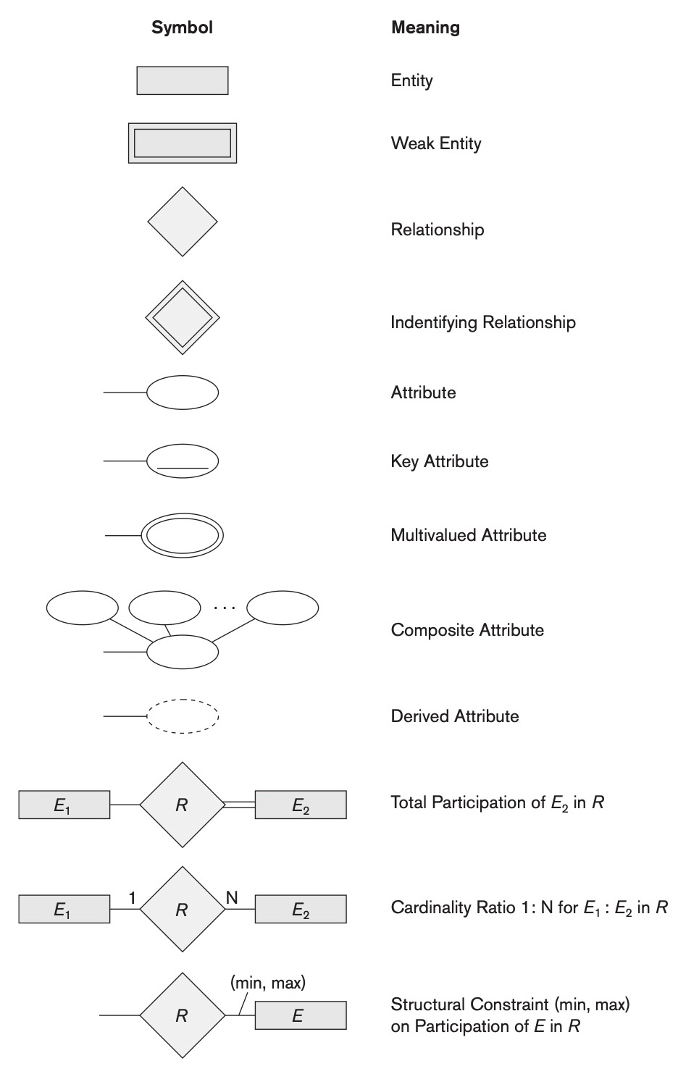
\includegraphics[width=0.7\textwidth]{images/legend.png}
  \caption{\textit{Legend of ER Diagram Symbols}}
\end{figure}
\begin{landscape}
  \section{ER Diagram for the NexStore Database}
  \begin{figure}[H]
    \centering
    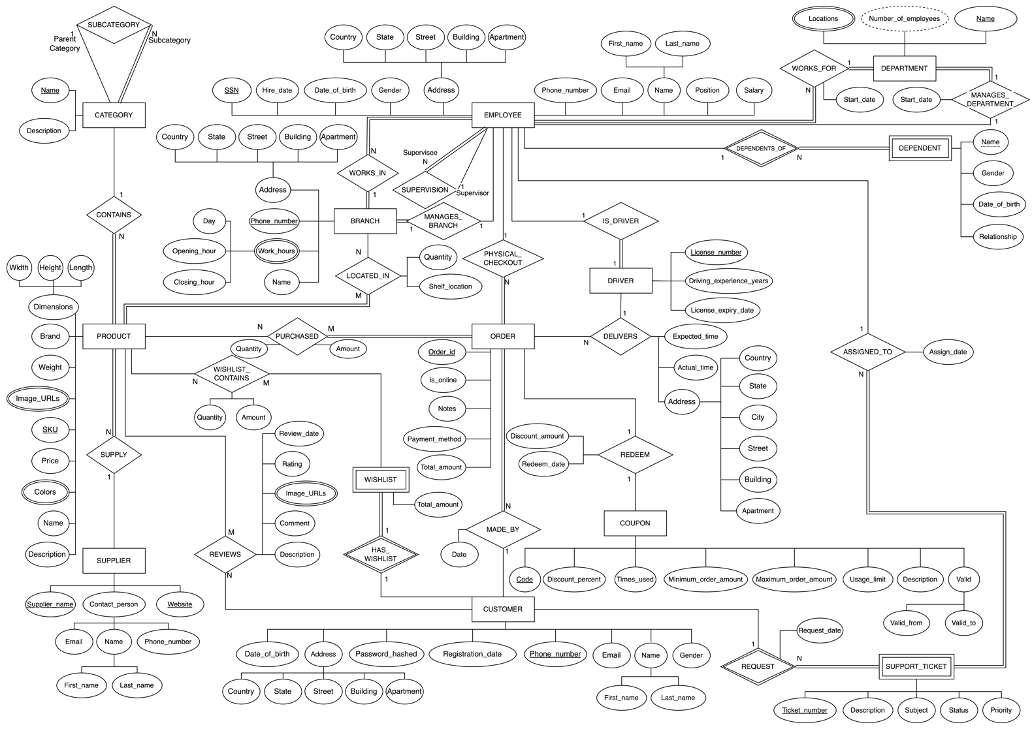
\includegraphics[width=1\textwidth]{images/diagrams/old-diagram.drawio.png}
    \caption{\textit{ER Diagram for the NexStore Database}}
  \end{figure}
\end{landscape}
\begin{landscape}
  \section{New Complete Amended ER Diagram for the NexStore Database}
  \begin{figure}[H]
    \centering
    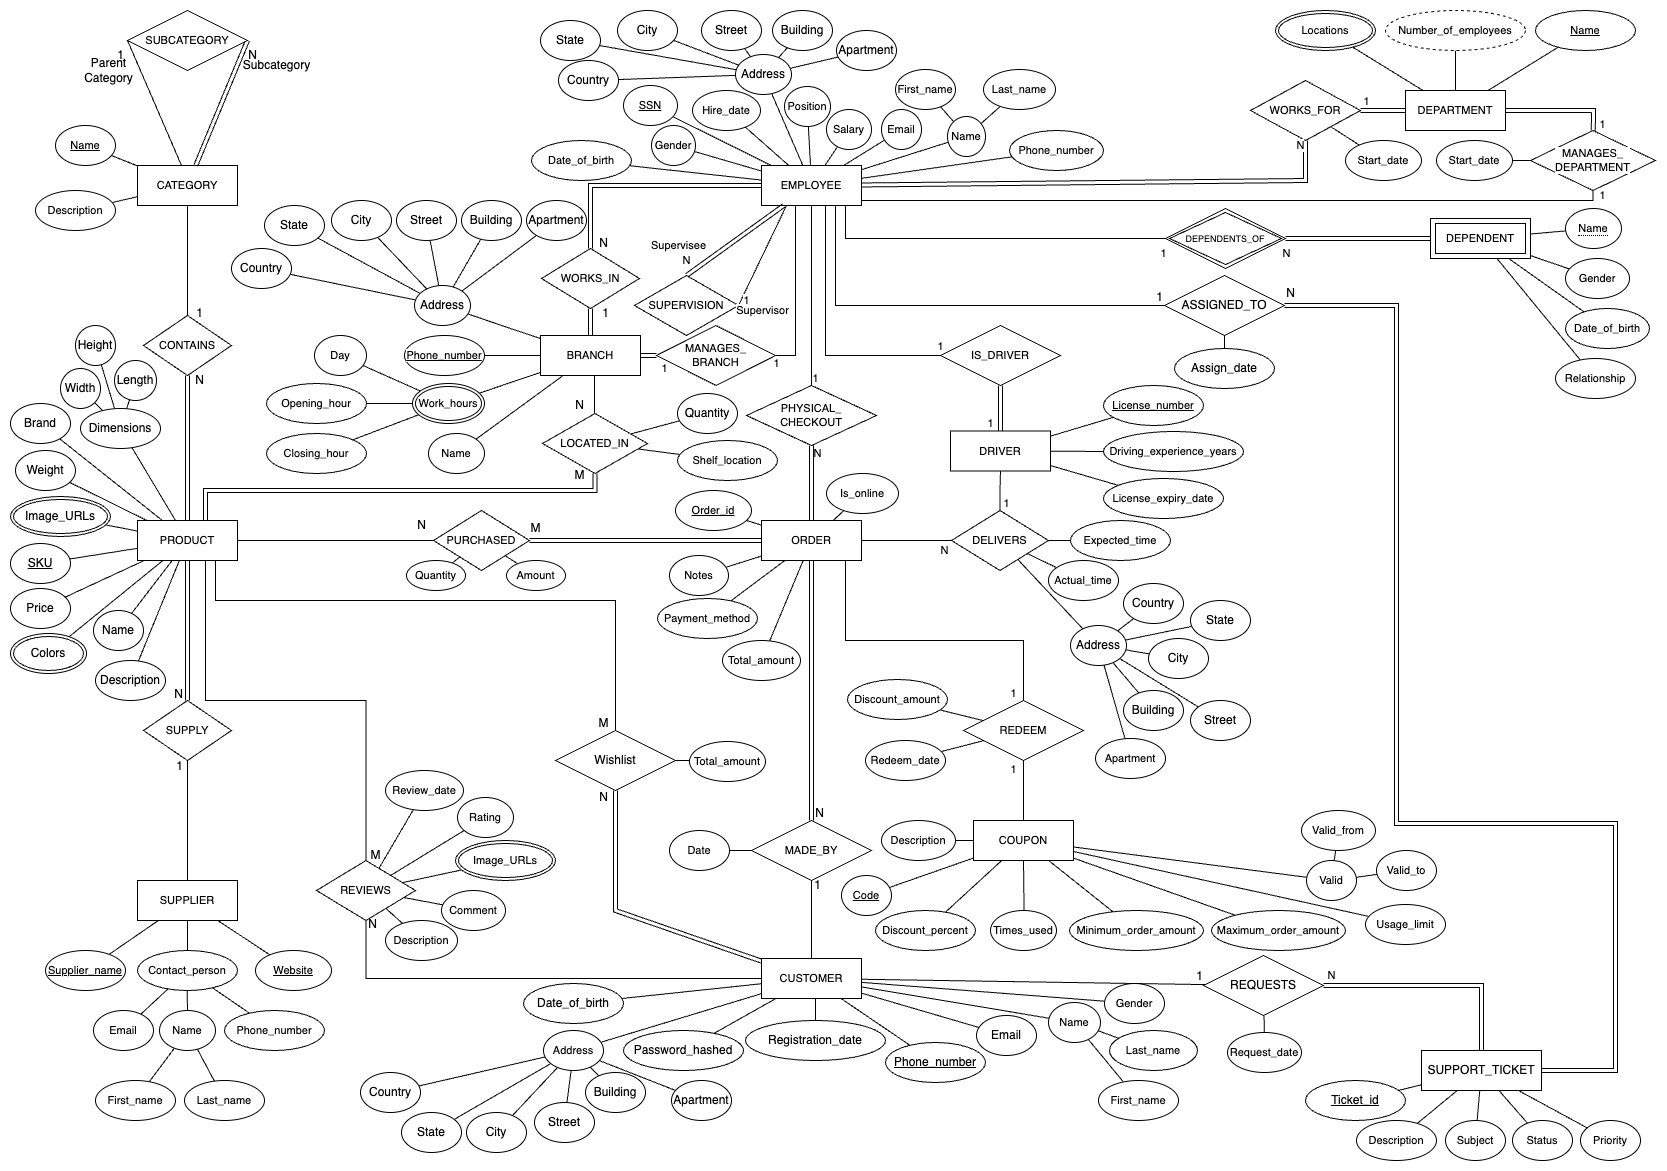
\includegraphics[width=1\textwidth]{images/diagrams/diagram.drawio.png}
    \caption{\textit{ER Diagram for the NexStore Database}}
  \end{figure}
\end{landscape}

\subsection{Entity Types and Their Attributes}

\subsubsection{Branch}
\begin{figure}[H]
  \centering
  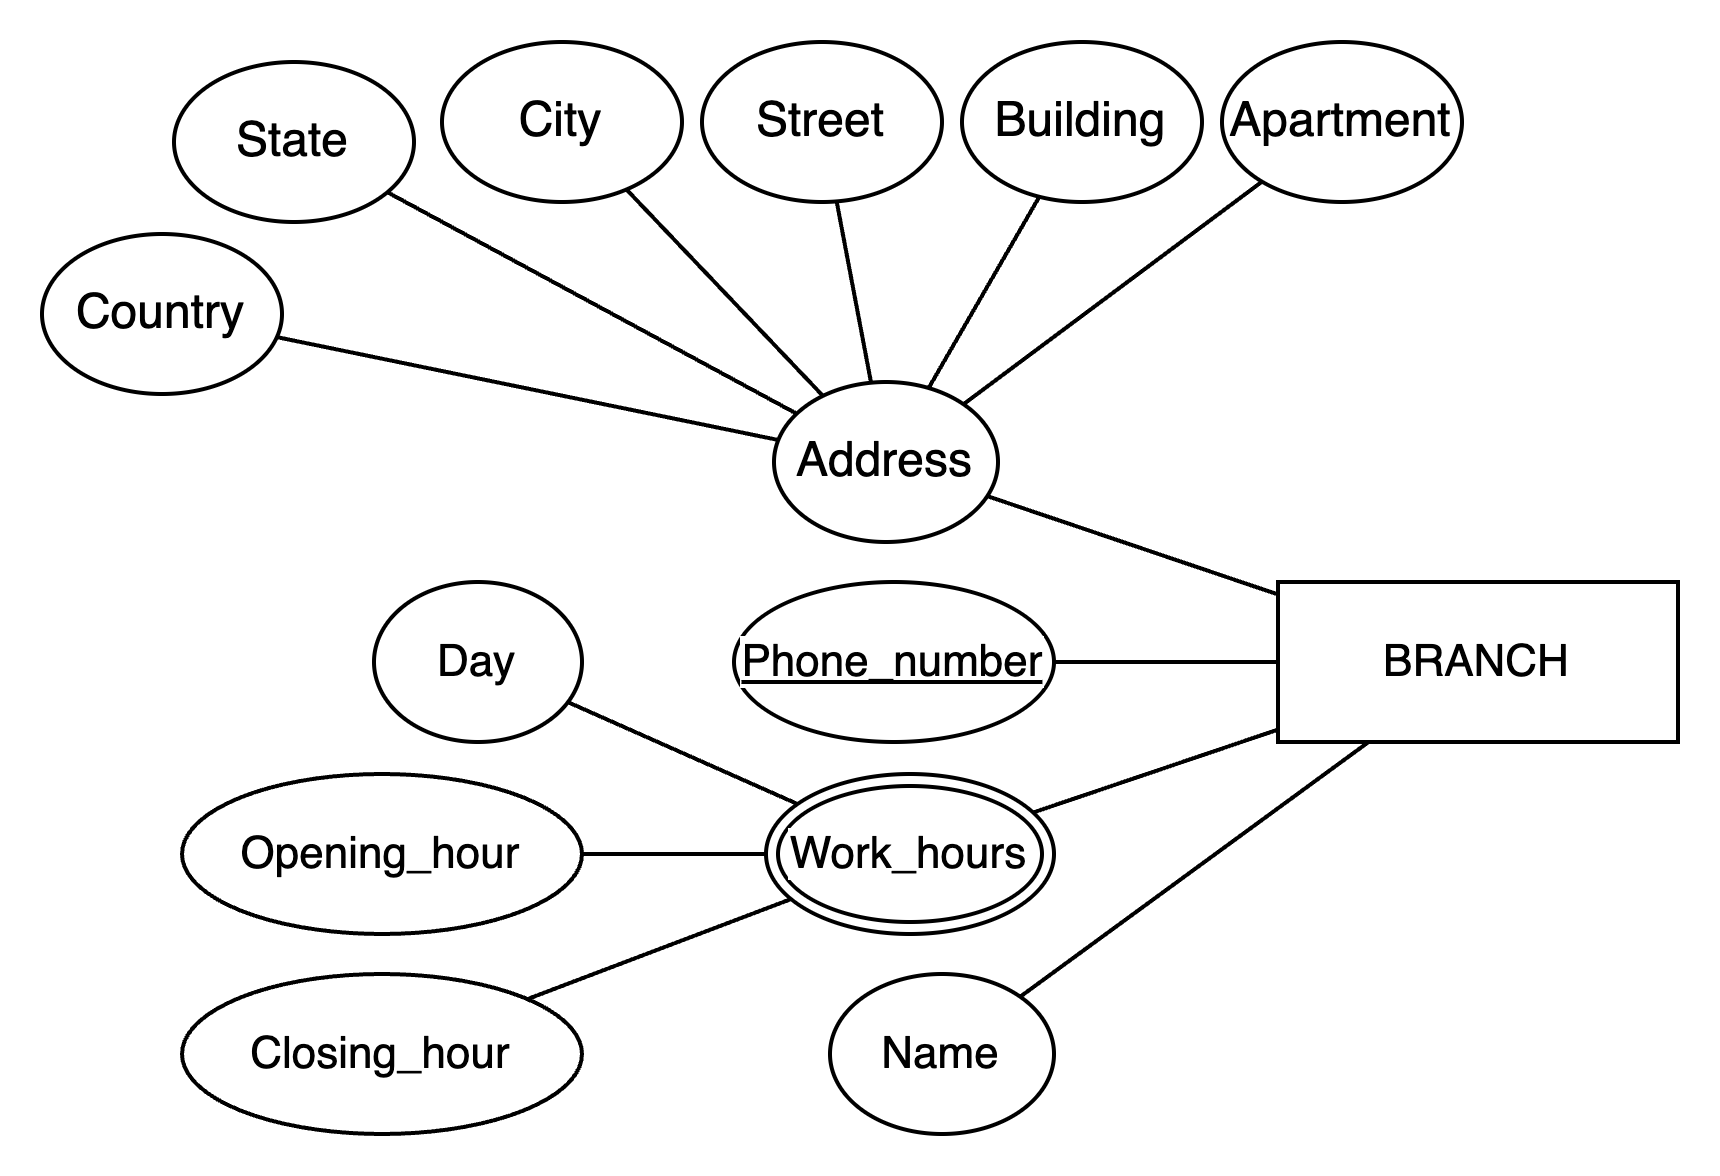
\includegraphics[width=0.7\textwidth]{images/entities/branch.png}
  \caption{\textit{Branch Entity and its Attributes}}
\end{figure}

The branch is one of the main entities presented in the ER diagram. The phone number was the primary key chosen to uniquely identify each branch. Additionally, the work hours were selected to be a composite multi-valued attribute since each branch might have different work hours depending on the weekday (e.g., weekends have different work hours). It comprises the weekday and the opening and closing hours of the branch. We included the composite attribute address to indicate the accurate address of the branch. Finally, we added the name attribute that indicates the name of each branch.

\subsubsection{Category}
\begin{figure}[H]
  \centering
  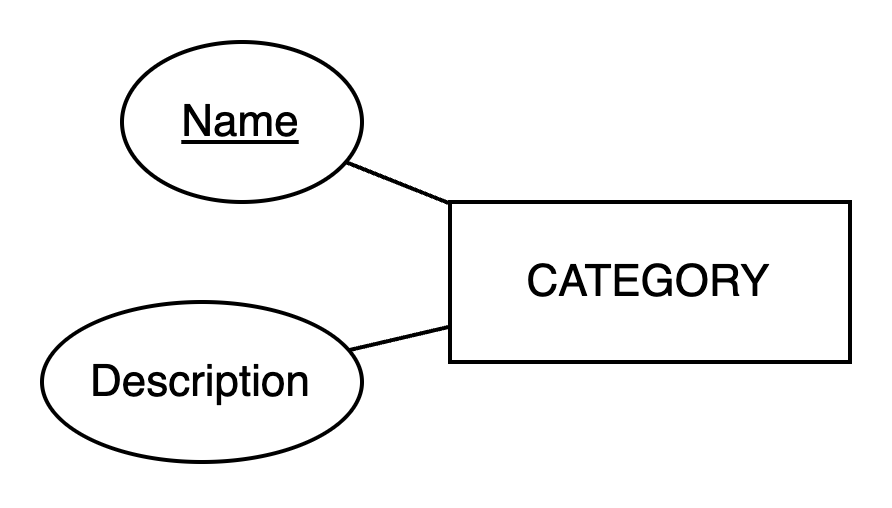
\includegraphics[width=0.6\textwidth]{images/entities/category.png}
  \caption{\textit{Category Entity and its Attributes}}
\end{figure}

As it is essential to know the category of each product, we include the category entity. It contains the Name of the category as a primary key in addition to the description of the category.

\subsubsection{Coupon}
\begin{figure}[H]
  \centering
  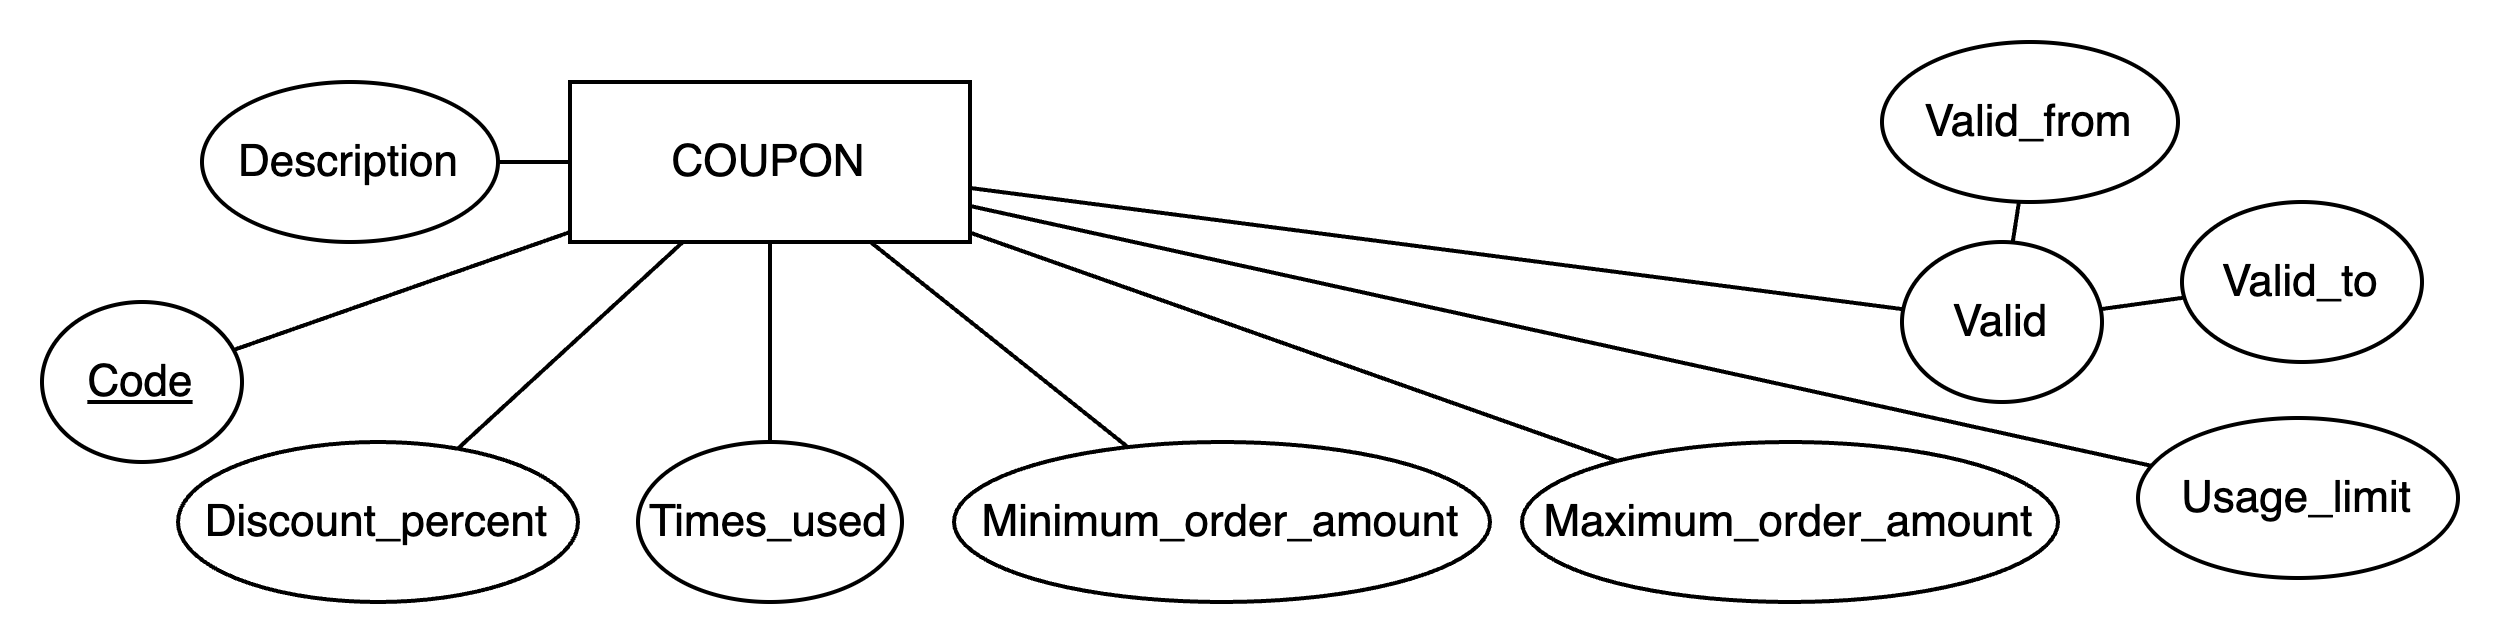
\includegraphics[width=0.7\textwidth]{images/entities/coupon.png}
  \caption{\textit{Coupon Entity and its Attributes}}
\end{figure}

In several events, a coupon might be applied to the order. The coupon can be identified by its unique code, so we chose the code to be the key attribute. Each coupon can be applied a certain number of times on a specific amount ranging from a minimum to a maximum, so we added the four attributes: "Times used", "Usage limit"," Minimum order amount" and "Maximum order amount". Furthermore, since each coupon is valid for a specific time interval, we included the "Valid to" and "Valid from" attributes. Finally, we added the attributes "Discount percent" and "Description" to indicate the discount percentage and the description of each coupon.

\subsubsection{Customer}
\begin{figure}[H]
  \centering
  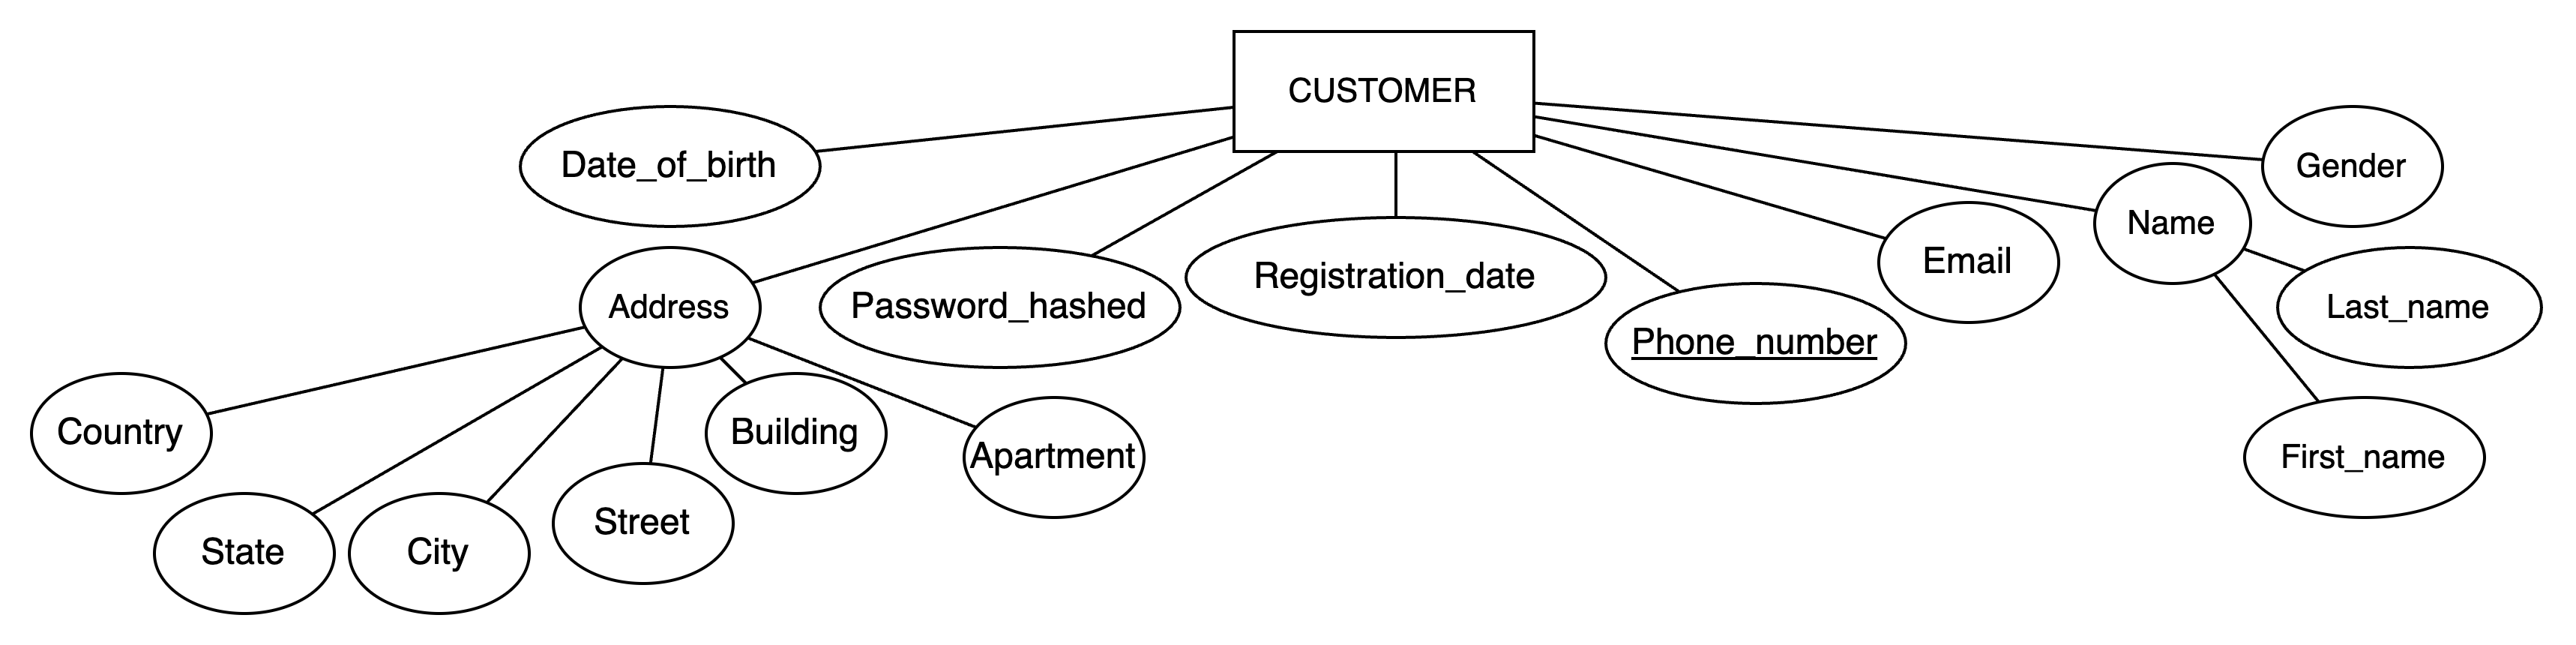
\includegraphics[width=0.7\textwidth]{images/entities/customer.png}
  \caption{\textit{Customer Entity and its Attributes}}
\end{figure}

This entity describes all the information we need to know about the customer comprising several attributes. We chose the phone number of the customer to be the primary key since it uniquely identifies each customer. Additionally, we included the name of the customer as a composite attribute as it contains the first and last name. Similarly, we added the address attribute that consists of the county, state, city, street, building, and apartment of the customer. Moreover, we added the password hashed to ensure security. Furthermore, we added the email attribute to ensure communication between the customer and the store. Finally, we added the gender, registration date, and date of birth of the customer that can be used for special events such as the customer's birthday.

\subsubsection{Department}
\begin{figure}[H]
  \centering
  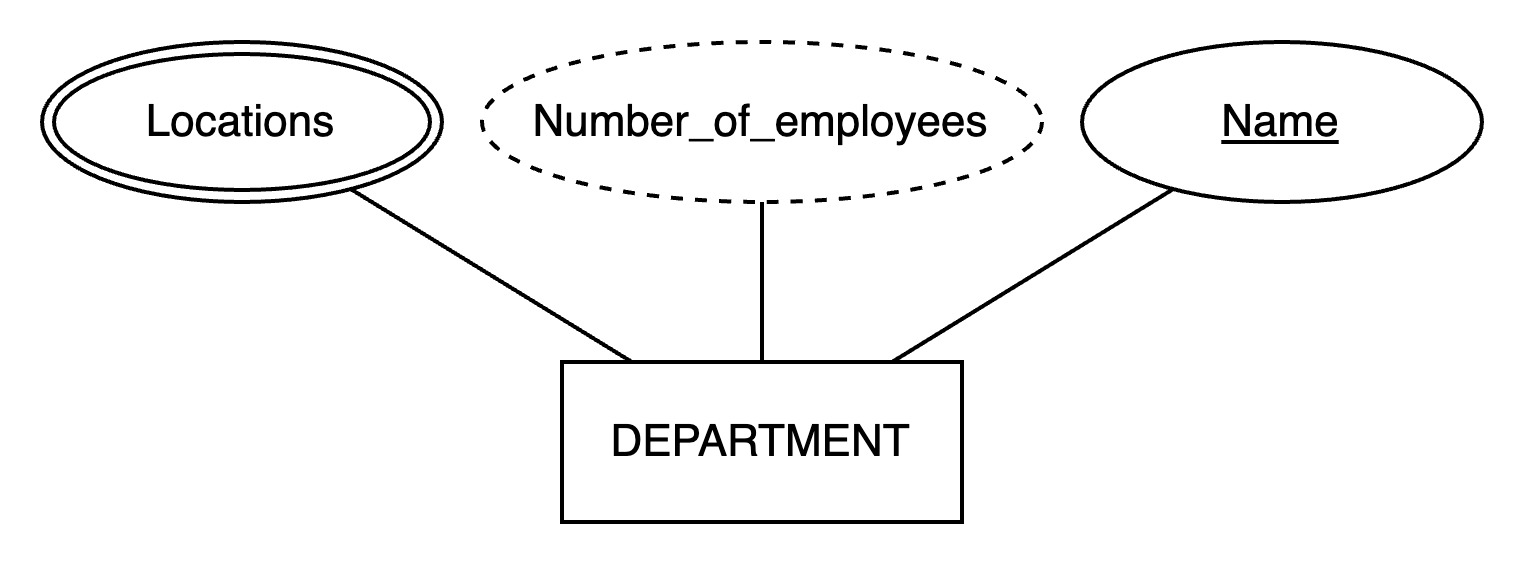
\includegraphics[width=0.7\textwidth]{images/entities/department.png}
  \caption{\textit{Department Entity and its Attributes}}
\end{figure}

This entity represents the departments in the company. Each department might have several locations, so this attribute was multi-valued. Since each department has a unique name, we chose the name to be the key attribute. Finally, we added the derived attribute "number of employees" to keep track of the updated number of employees in each department.

\subsubsection{Dependent}
\begin{figure}[H]
  \centering
  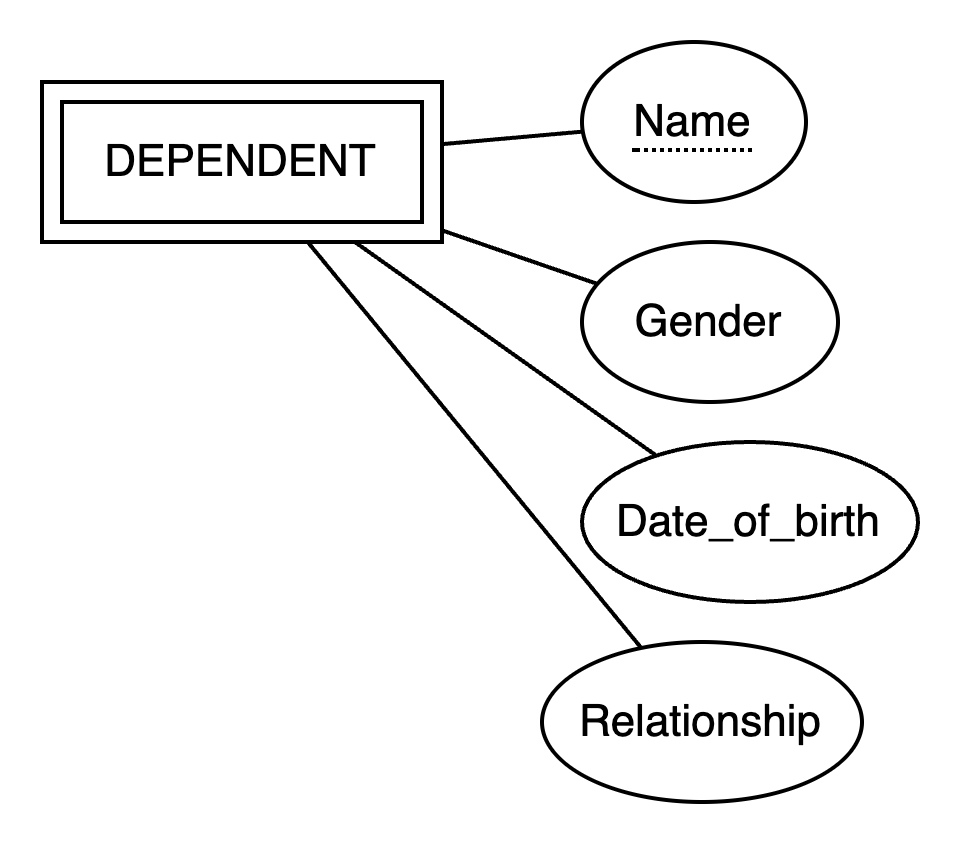
\includegraphics[width=0.7\textwidth]{images/entities/dependent.png}
  \caption{\textit{Dependent Entity and its Attributes}}
\end{figure}

Each employee has dependents that are related to them. Since we cannot have a dependent without having an employee, we set the dependent entity to be weak with the name attribute as a weak attribute of it.

\subsubsection{Driver}
\begin{figure}[H]
  \centering
  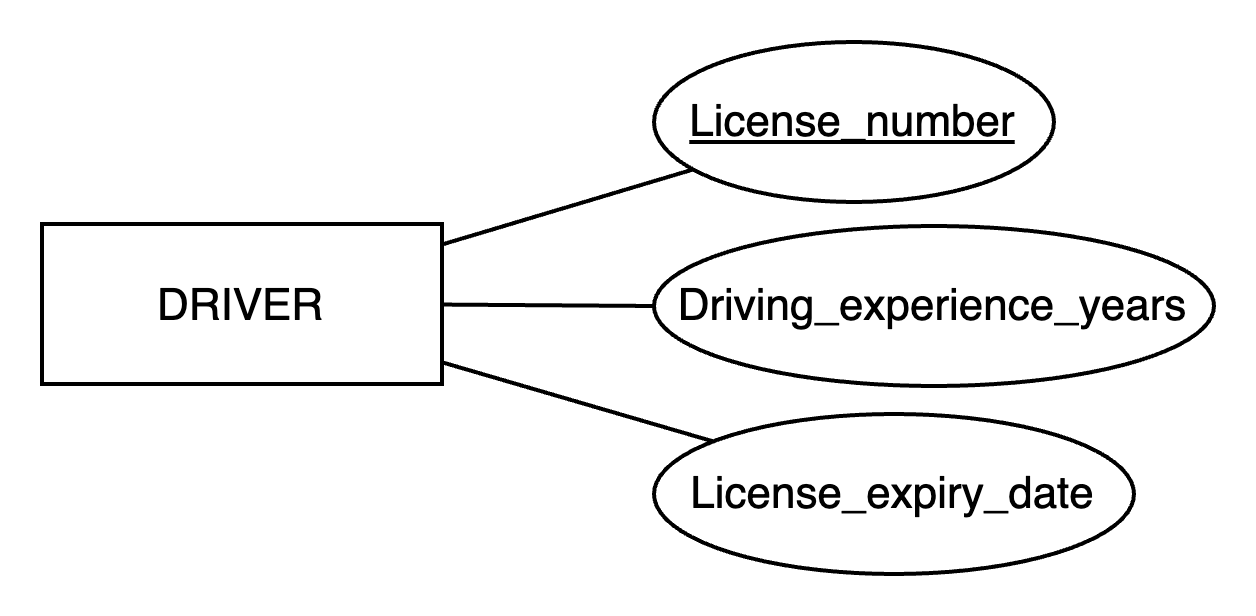
\includegraphics[width=0.7\textwidth]{images/entities/driver.png}
  \caption{\textit{Driver Entity and its Attributes}}
\end{figure}

To deliver an online order, a driver needs to be assigned. This driver entity has the license number as a primary key since it uniquely identifies the driver. Additionally, other attributes reflecting information about the driver are the driving experience years and the license expiry date.

\subsubsection{Employee}
\begin{figure}[H]
  \centering
  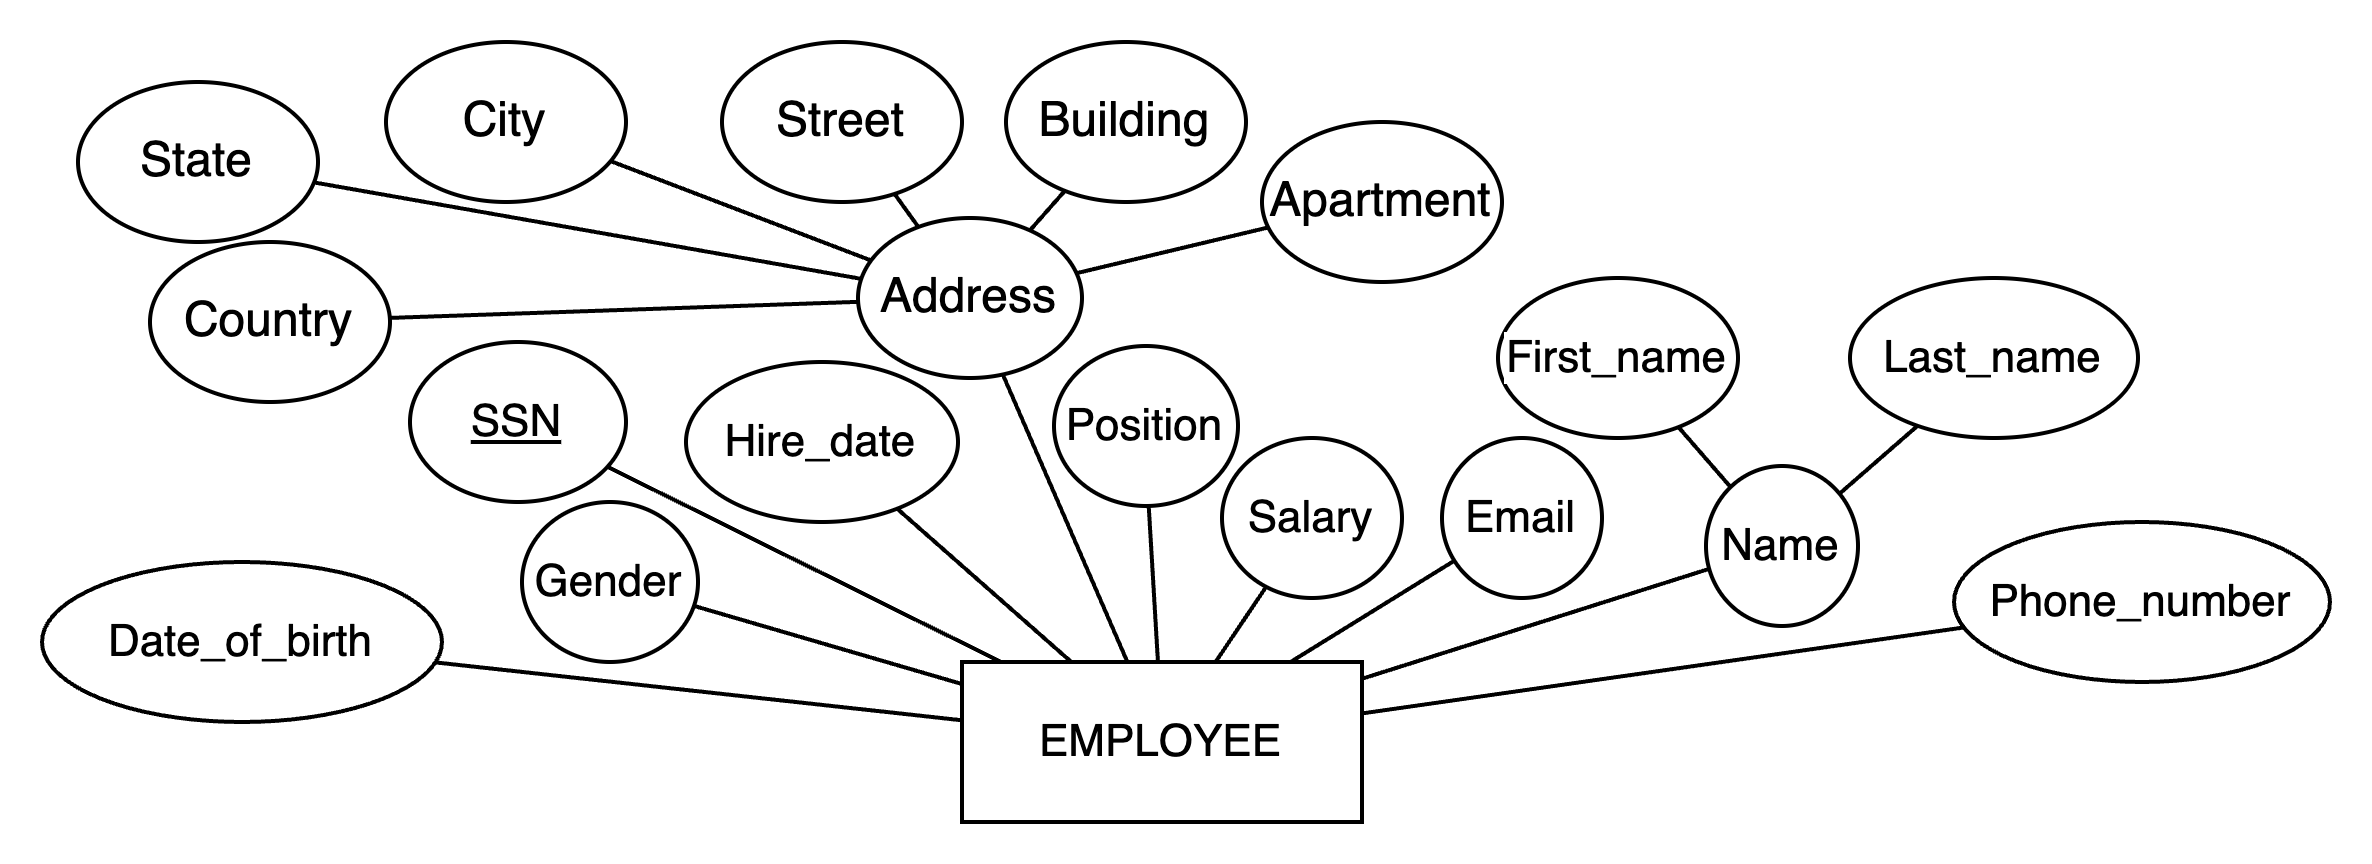
\includegraphics[width=0.7\textwidth]{images/entities/employee.png}
  \caption{\textit{Employee Entity and its Attributes}}
\end{figure}

One of the basic entities in this project is the employee entity which portrays all the information needed about the employee. We chose the social security number (SSN) of the employee as the primary key since it uniquely identifies each employee. Additionally, we added the address attribute that consists of the county, state, city, street, building, and apartment of the employee. Moreover, we included the name of the customer as a composite attribute as it contains the first and last name. Finally, we added all the information needed such as date of birth, phone number, position, gender, email address, salary, and hire date to keep an eye on this important personal information.

\subsubsection{Order}
\begin{figure}[H]
  \centering
  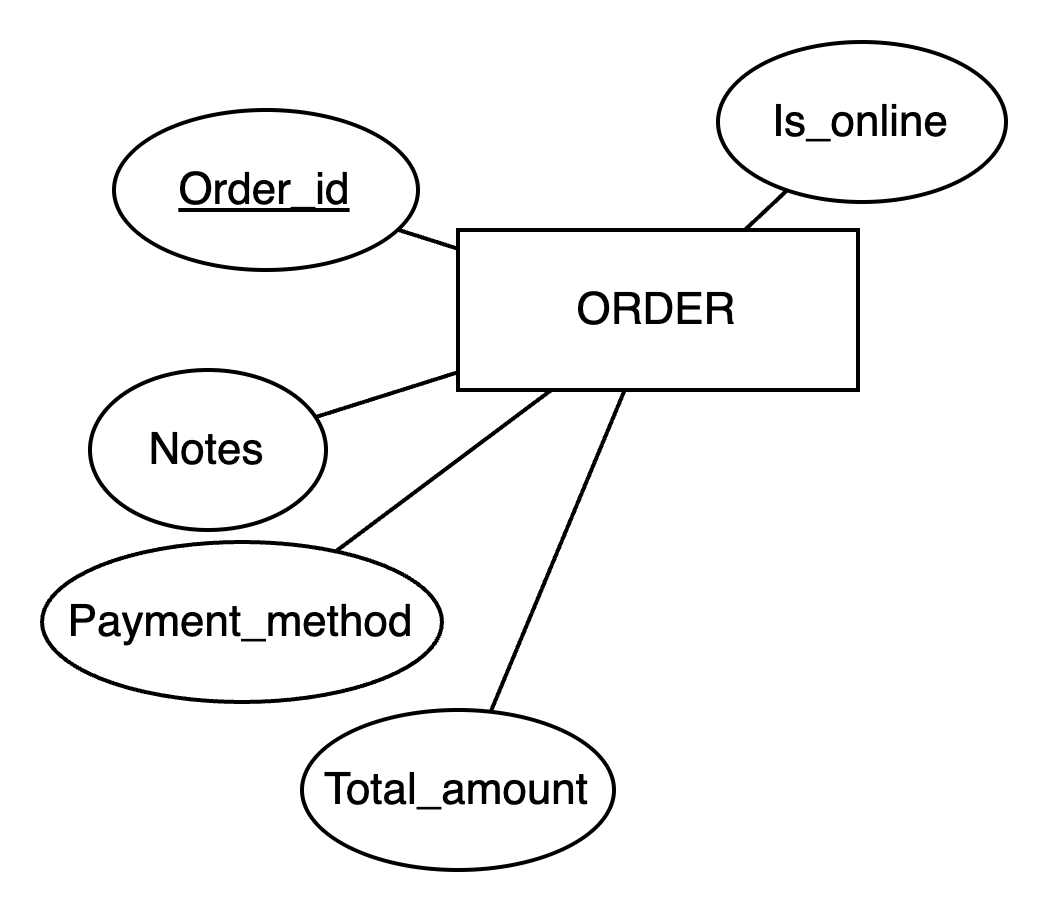
\includegraphics[width=0.7\textwidth]{images/entities/order.png}
  \caption{\textit{Order Entity and its Attributes}}
\end{figure}

To proceed with the customers' orders on both physical and online channels, the order entity was added. The primary key of this entity is the unique order ID. Other attributes include the total cost of the order, the payment method used, and any notes for this order. Finally, we added the "is online" attribute to specify whether the order was conducted physically or online.

\subsubsection{Product}
\begin{figure}[H]
  \centering
  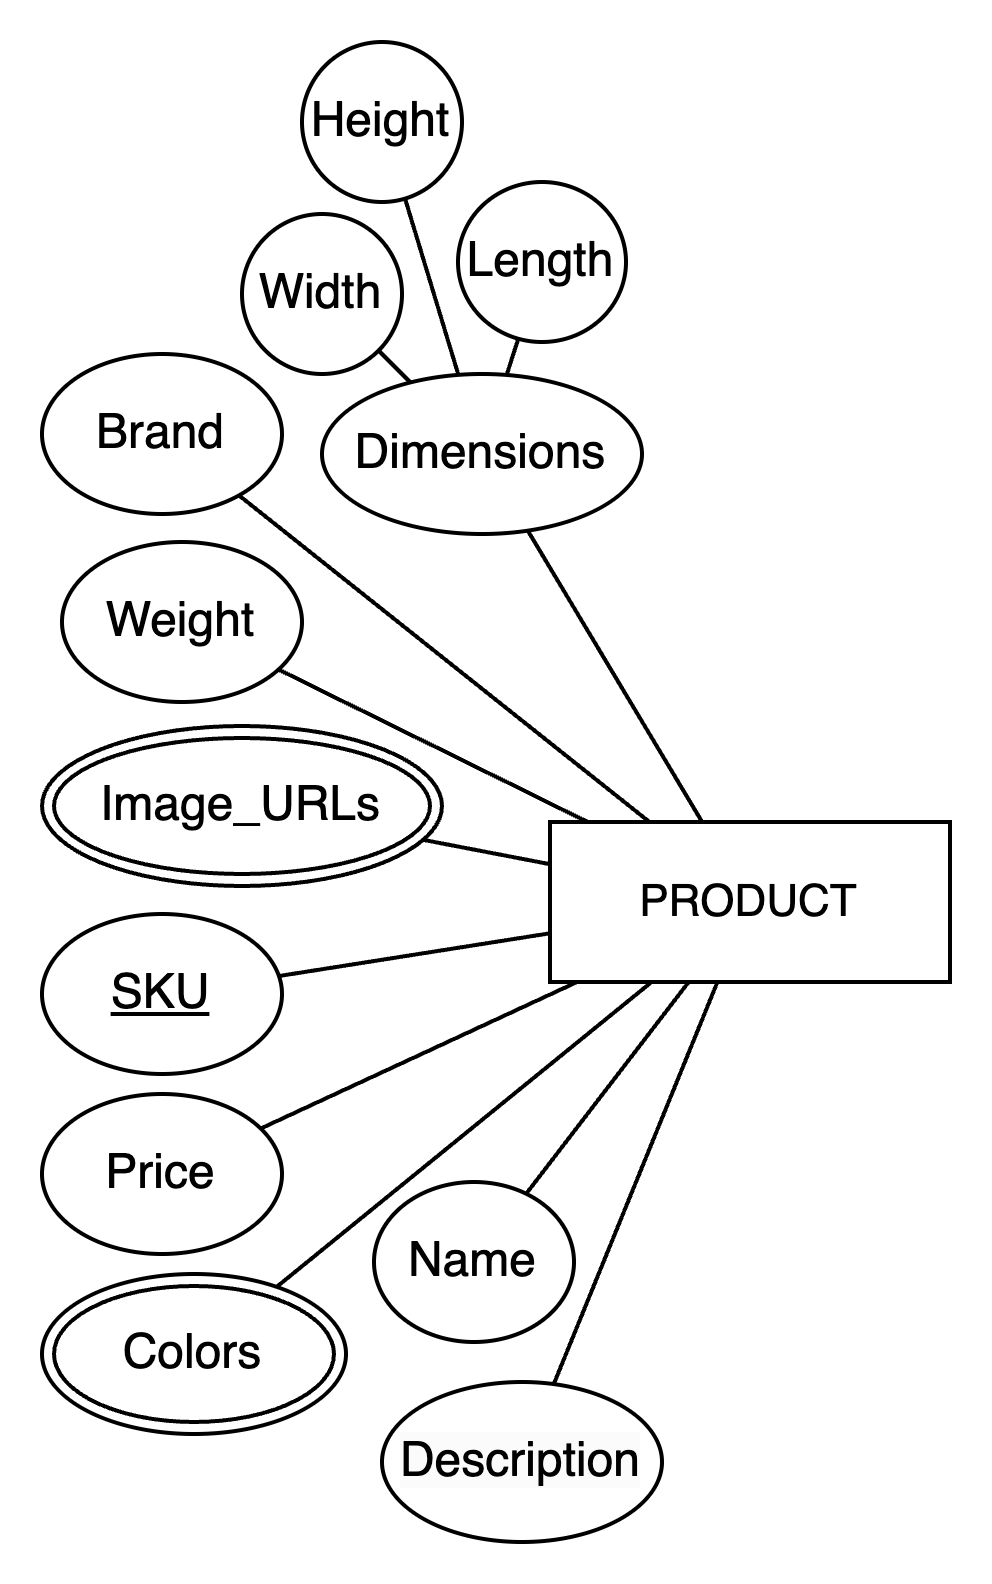
\includegraphics[width=0.7\textwidth]{images/entities/product.png}
  \caption{\textit{Product Entity and its Attributes}}
\end{figure}

This product entity describes all the information we need to know about the product comprising several attributes. We set the product entity as a weak entity since it doesn't exist without the dependence on the branch entity. We chose the stock-keeping unit (SKU) of the product as the primary key since it uniquely identifies each product. Additionally, we included the dimensions of the product as a composite attribute as it contains the height, width, and length of the product. Moreover, we added the colors as a multi-valued attribute since one product could have various colors. Similarly, we added the image URLs as a multi-valued attribute since a product could have several images to cast it online. Furthermore, we added the weight to keep track of the total weight of the shipment. In addition, we used the quantity to view the available amount of this product. Finally, we added the name, description, price, brand, and the date when the product was added to specify these essential parameters of each product.

\subsubsection{Supplier}
\begin{figure}[H]
  \centering
  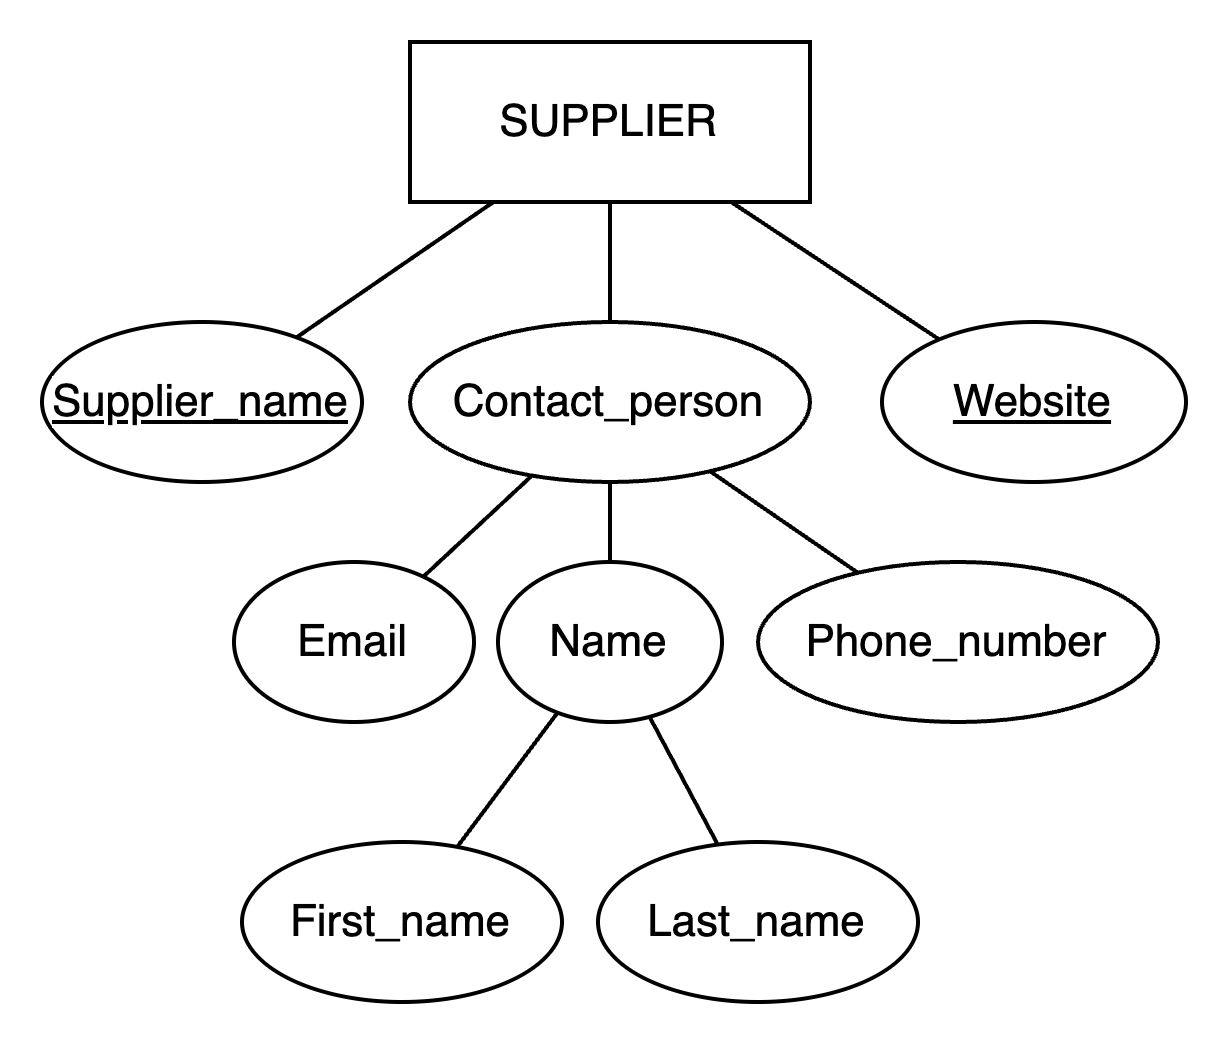
\includegraphics[width=0.7\textwidth]{images/entities/supplier.png}
  \caption{\textit{Supplier Entity and its Attributes}}
\end{figure}

Another basic entity in this project is the supplier entity which shows all the information needed about the employee. We chose the supplier's website and name as the primary keys since they uniquely identify each supplier. Finally, we included the contacted person as a composite attribute as it contains a composite attribute, the name composing the first and last name, email, and supplier's phone number.

\subsubsection{Support Ticket}
\begin{figure}[H]
  \centering
  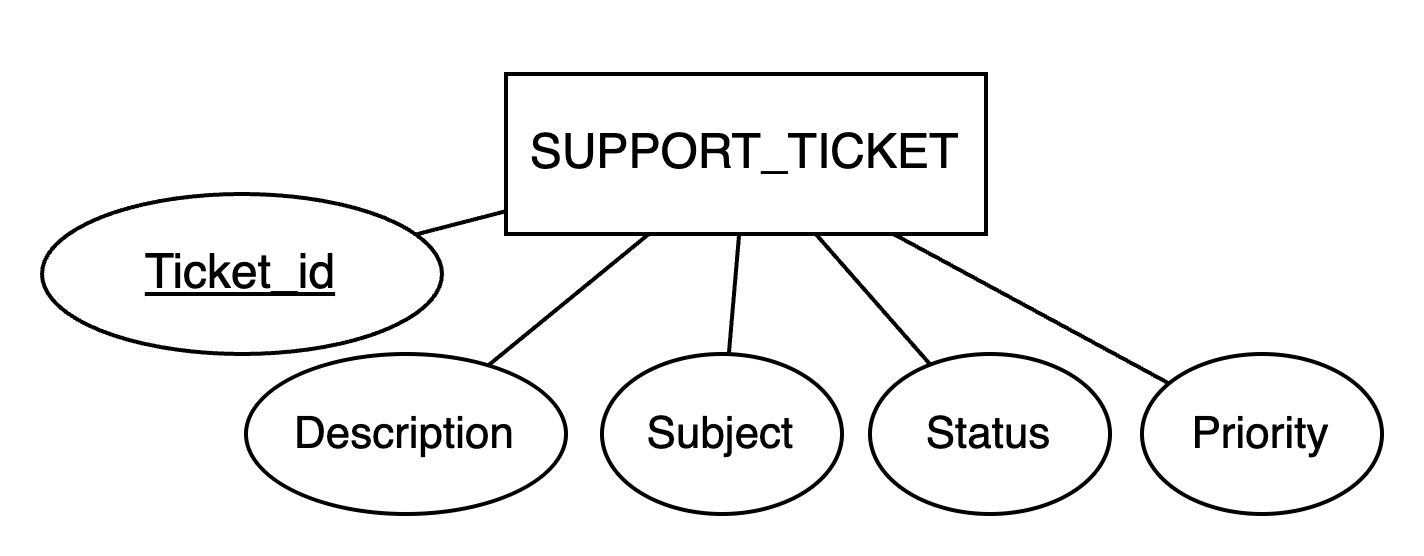
\includegraphics[width=0.7\textwidth]{images/entities/support_ticket.png}
  \caption{\textit{Support Ticket Entity and its Attributes}}
\end{figure}

To keep up with the customers' complaints, a support ticket entity was needed. We used the ticket ID as a primary key as it uniquely identifies the support ticket. Moreover, other attributes like subject, description, priority -to know how urgent the request is-, and status to keep track of it were needed.

\subsection{Relationships and their Explanations}

\subsubsection{Assigned To}
\begin{figure}[H]
  \centering
  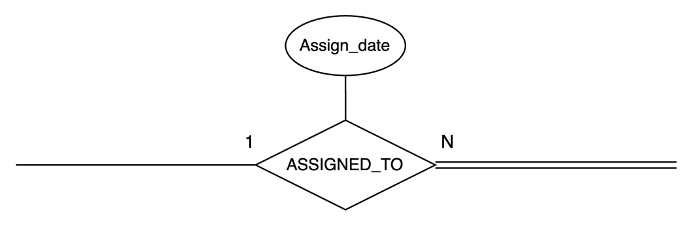
\includegraphics[width=0.7\textwidth]{images/relationships/assigned_to.png}
  \caption{\textit{Assigned To Relationship}}
\end{figure}

The relationship "assigned to" is between the employee and the support ticket. It maps the employee to zero or more support tickets and stores the data of the assignment. Also, it supports the real-life need that a support ticket must be assigned to an employee.

\subsubsection{Contains}
\begin{figure}[H]
  \centering
  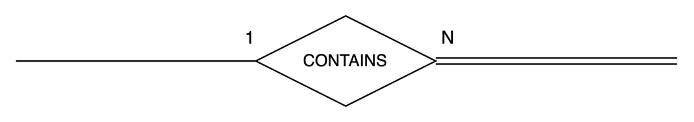
\includegraphics[width=0.7\textwidth]{images/relationships/contains.png}
  \caption{\textit{Contains Relationship}}
\end{figure}

The relationship "contains" is between a category and products. A category may contain many products. This organized the products the company has by categorizing all the products under specific categories. Also, it helps a better user experience by searching the category and then looking for the specific product needed in the category.

\subsubsection{Delivers}
\begin{figure}[H]
  \centering
  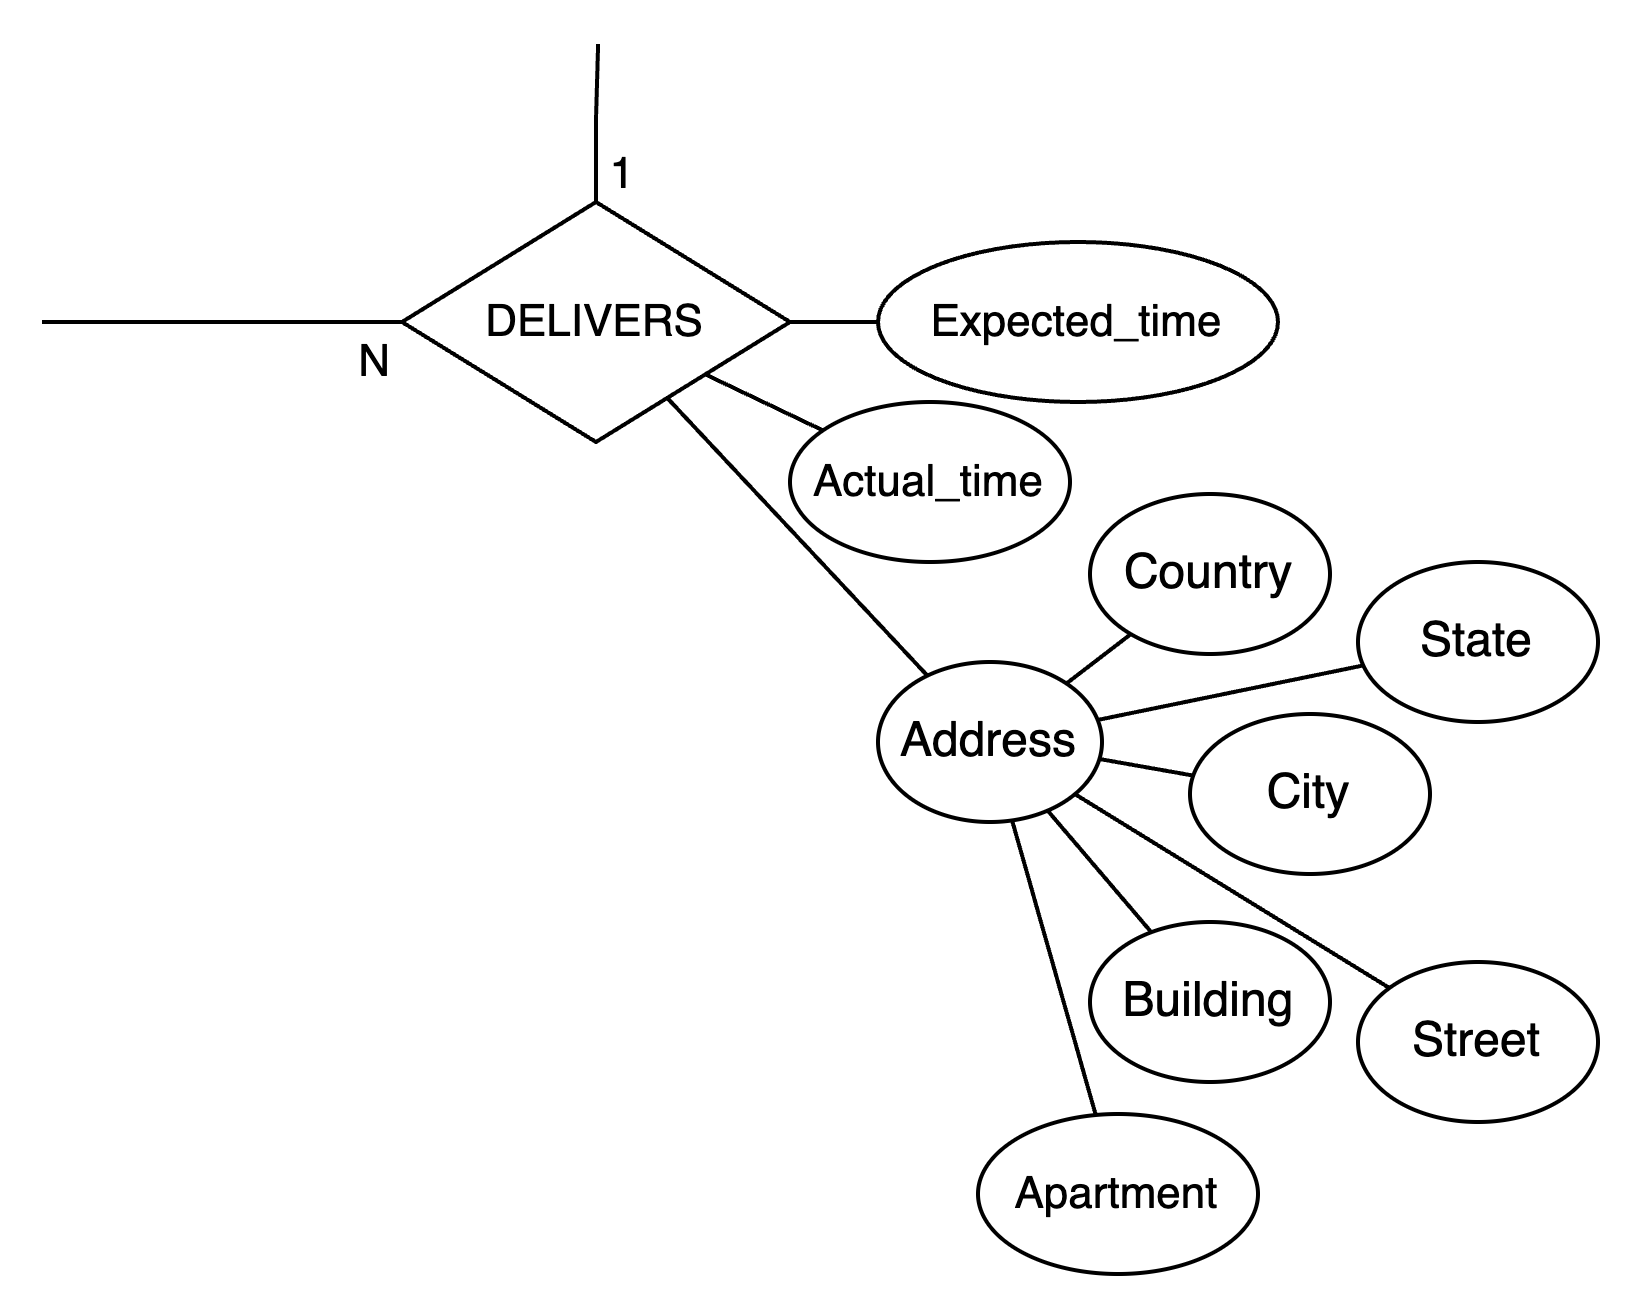
\includegraphics[width=0.7\textwidth]{images/relationships/delivers.png}
  \caption{\textit{Delivers Relationship}}
\end{figure}

The relationship "Delivers" is between the Driver and the Order. The driver is responsible for delivering the order to the requested address provided by the customer. It includes the "expected time" attribute to be displayed to the customer and the "actual time" attribute to help predict accurate delivery times for future orders. A driver can deliver many orders, but each order is delivered by one driver. Some orders may be physically checked out, in which case no delivery is required.

\subsubsection{Dependents Of}
\begin{figure}[H]
  \centering
  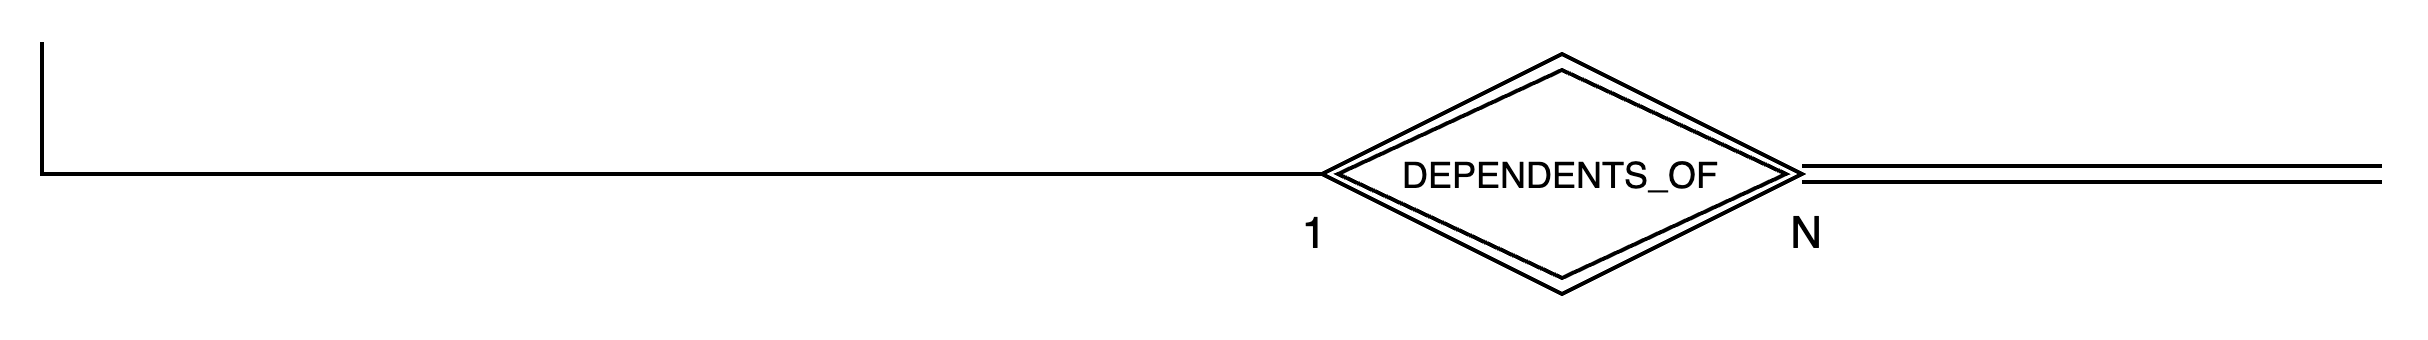
\includegraphics[width=0.7\textwidth]{images/relationships/dependents_of.png}
  \caption{\textit{Dependents Of Relationship}}
\end{figure}

The "Dependents Of" relationship is between the Employee and the Dependent. Each employee may have several dependents. This relationship is essential for connecting employees to their dependents, who might be insured by the company in the future.

\subsubsection{Is Driver}
\begin{figure}[H]
  \centering
  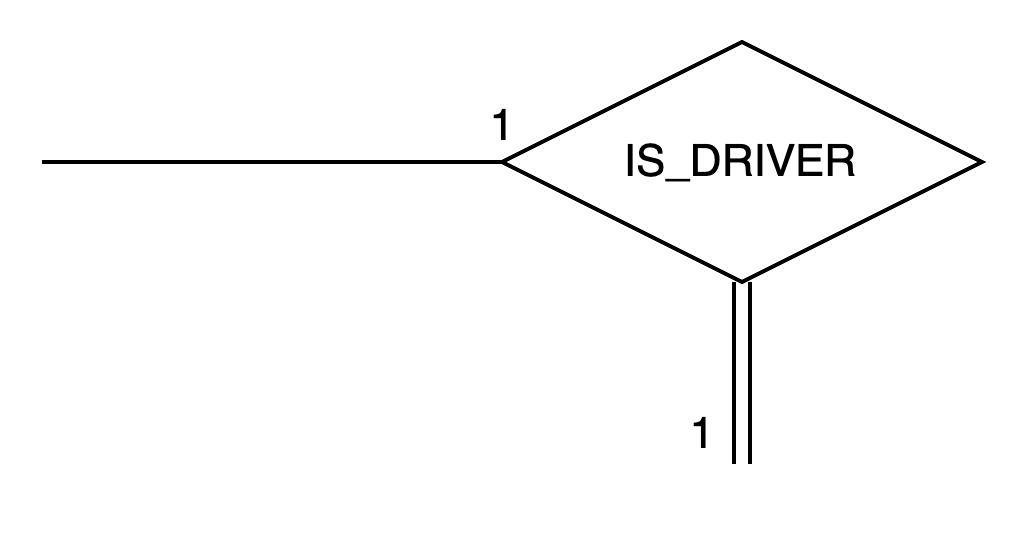
\includegraphics[width=0.7\textwidth]{images/relationships/is_driver.png}
  \caption{\textit{Is Driver Relationship}}
\end{figure}

The "Is Driver" relationship is between the Employee and the Driver. Each driver is also an employee of the company, and this relationship helps categorize employees based on whether they are drivers.

\subsubsection{Located In}
\begin{figure}[H]
  \centering
  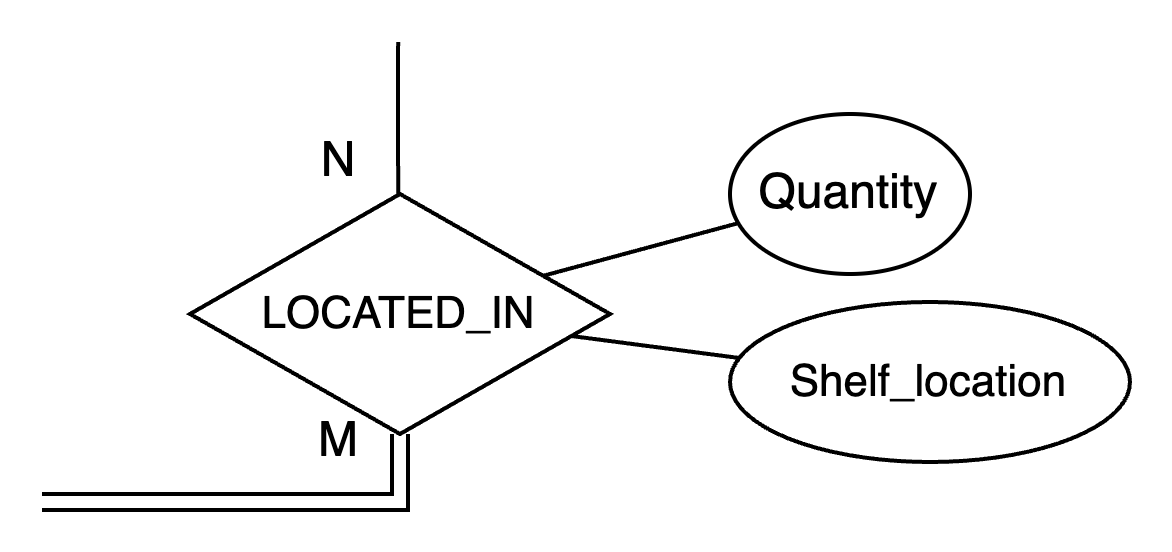
\includegraphics[width=0.7\textwidth]{images/relationships/located_in.png}
  \caption{\textit{Located In Relationship}}
\end{figure}

The "Located In" relationship is between the Product and the Branch. A branch can stock multiple products, each with specific quantities placed on certain shelves. The quantity and shelf location may vary between branches to avoid redundancy.

\subsubsection{Made By}
\begin{figure}[H]
  \centering
  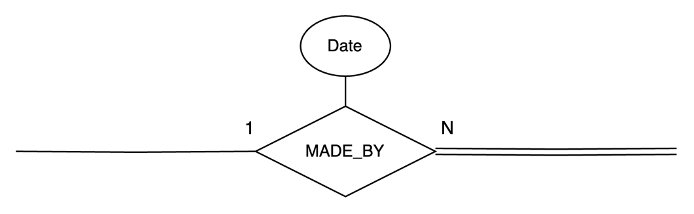
\includegraphics[width=0.7\textwidth]{images/relationships/made_by.png}
  \caption{\textit{Made By Relationship}}
\end{figure}

The "Made By" relationship connects the Customer and the Order. Each order is placed by one customer, but a customer can place multiple orders. This relationship also stores the order date for tracking purposes.

\subsubsection{Manages Branch}
\begin{figure}[H]
  \centering
  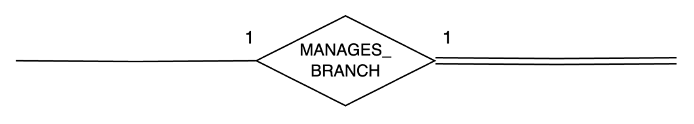
\includegraphics[width=0.7\textwidth]{images/relationships/manages_branch.png}
  \caption{\textit{Manages Branch Relationship}}
\end{figure}

The "Manages Branch" relationship is between the Employee and the Branch. Each branch is managed by one employee, but not all employees are managers. This relationship helps define the company's management structure.

\subsubsection{Manages Department}
\begin{figure}[H]
  \centering
  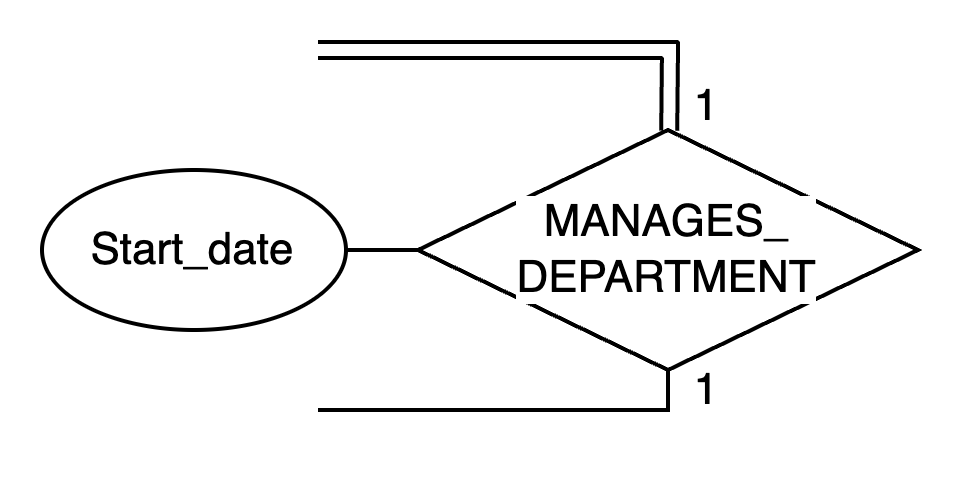
\includegraphics[width=0.7\textwidth]{images/relationships/manages_department.png}
  \caption{\textit{Manages Department Relationship}}
\end{figure}

The "Manages Department" relationship is between the Employee and the Department. An employee can manage one department, enabling a clear tracking of department managers.

\subsubsection{Physical Checkout}
\begin{figure}[H]
  \centering
  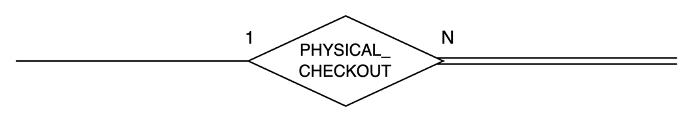
\includegraphics[width=0.7\textwidth]{images/relationships/physical_checkout.png}
  \caption{\textit{Physical Checkout Relationship}}
\end{figure}

The "Physical Checkout" relationship is between the Employee and the Order. Each order must be checked out by one employee, but an employee can check out multiple orders. This relationship prevents duplicate receipts and streamlines order management.

\subsubsection{Purchased}
\begin{figure}[H]
  \centering
  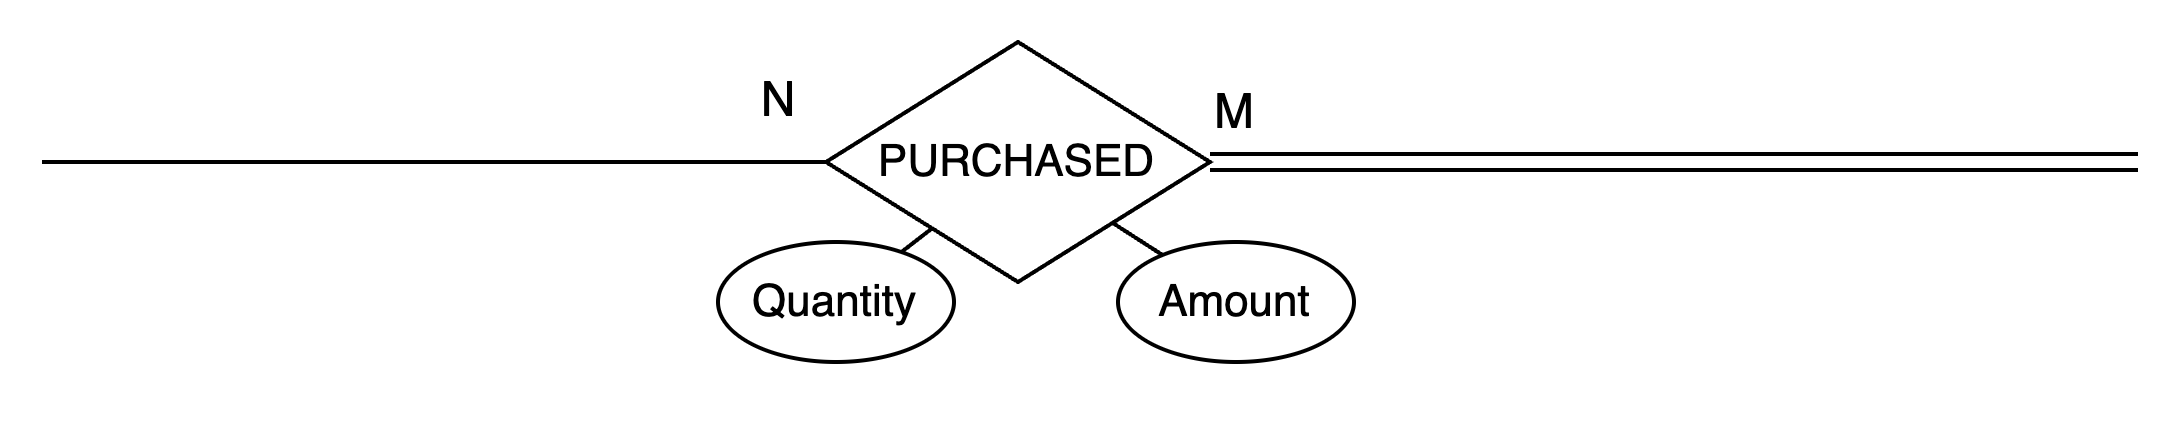
\includegraphics[width=0.7\textwidth]{images/relationships/purchased.png}
  \caption{\textit{Purchased Relationship}}
\end{figure}

The "Purchased" relationship is between the Product and the Order. An order can contain multiple products, each with specific quantities and prices. This relationship tracks these details to calculate the total order value.

\subsubsection{Redeem}
\begin{figure}[H]
  \centering
  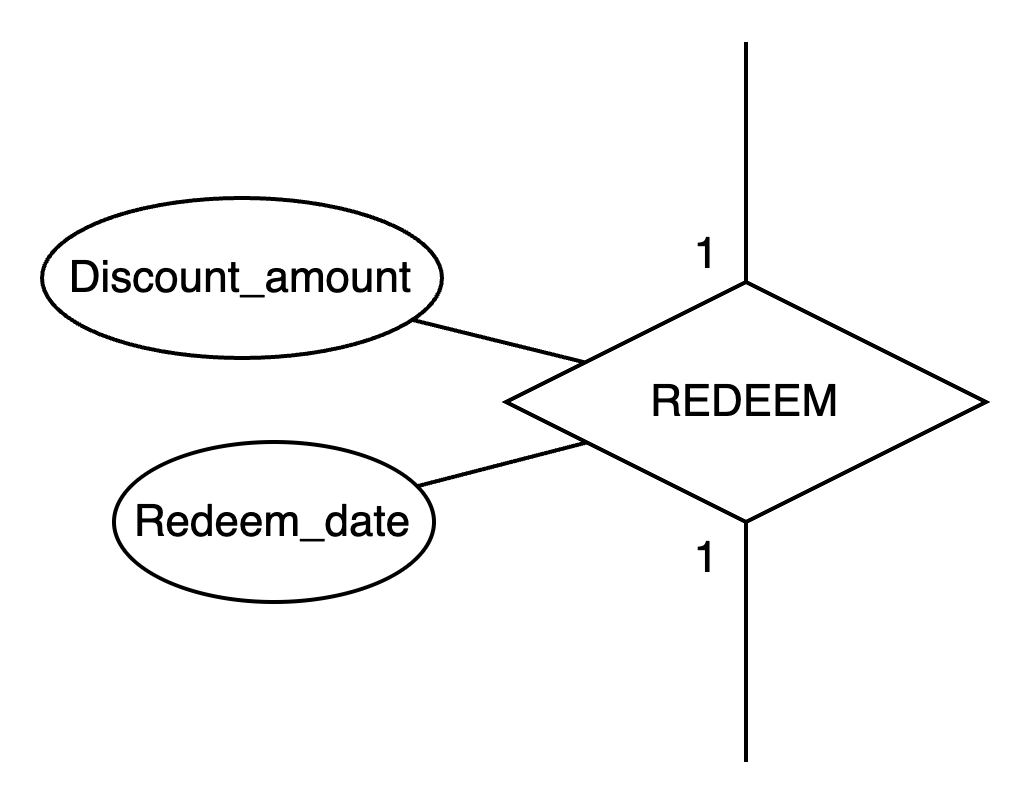
\includegraphics[width=0.6\textwidth]{images/relationships/redeem.png}
  \caption{\textit{Redeem Relationship}}
\end{figure}

The "Redeem" relationship connects the Order and the Coupon. An order can be redeemed using one coupon, and a coupon can only redeem one order. This relationship supports special occasion discounts.

\subsubsection{Request}
\begin{figure}[H]
  \centering
  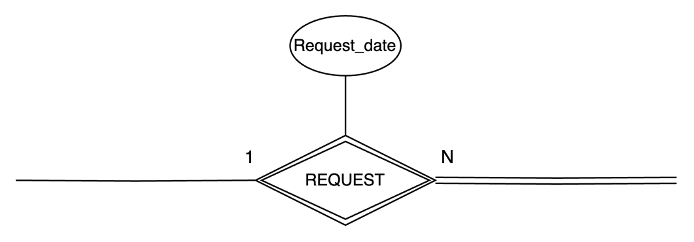
\includegraphics[width=0.7\textwidth]{images/relationships/request.png}
  \caption{\textit{Request Relationship}}
\end{figure}

This relationship is between the customer and the support ticket. It enables the customer to create various support tickets, but a ticket can't be created without the request of the customer. By including this relationship in our system, it manages the complaints of the customers efficiently.

\subsubsection{Reviews}
\begin{figure}[H]
  \centering
  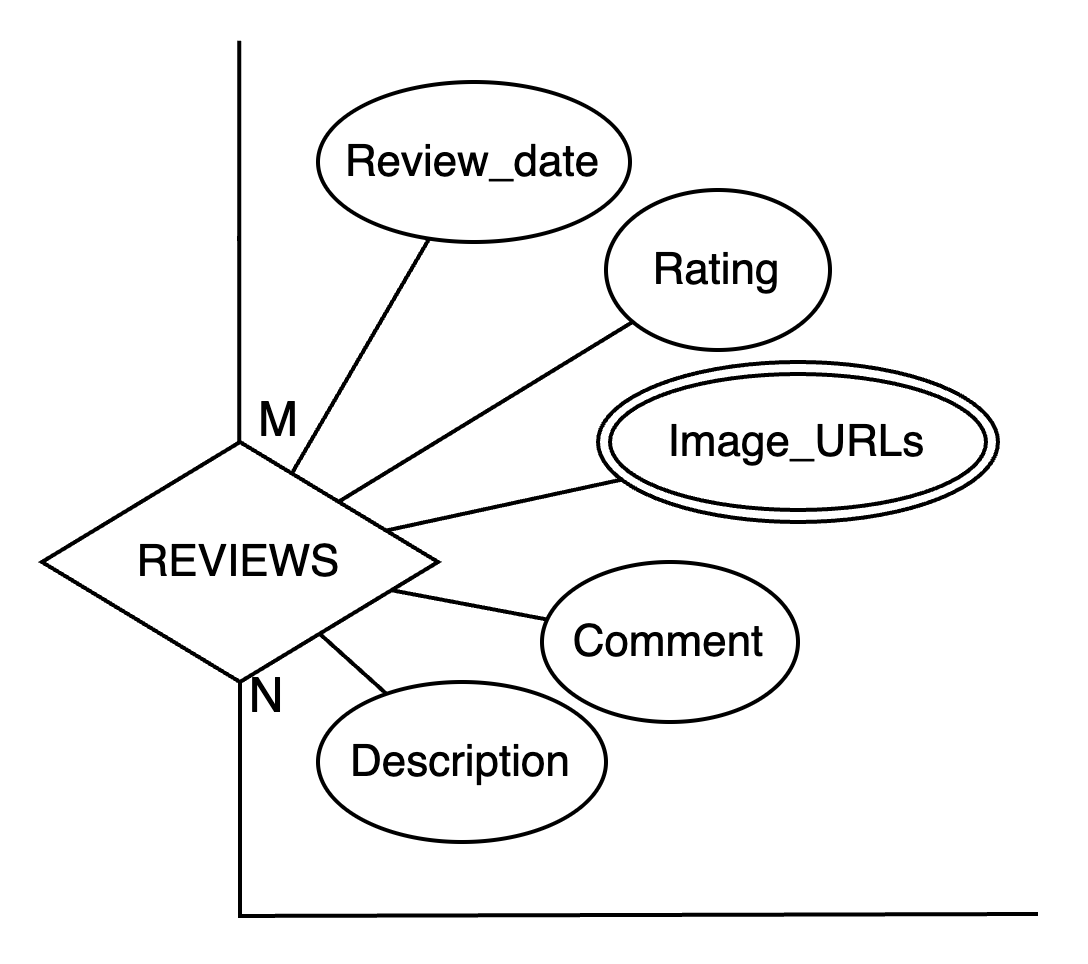
\includegraphics[width=0.7\textwidth]{images/relationships/reviews.png}
  \caption{\textit{Reviews Relationship}}
\end{figure}

The "Reviews" relationship connects the Customer and the Product. A customer can review several products, and a product can receive reviews from multiple customers. This helps gather feedback for product improvement.

\subsubsection{Subcategory}
\begin{figure}[H]
  \centering
  
\includegraphics[width=0.7\textwidth]{images/relationships/subcategory.png}
  \caption{\textit{Subcategory Relationship}}
\end{figure}

The "Subcategory" relationship connects a Category to its subcategories. This relationship ensures hierarchical organization of product categories.

\subsubsection{Supply}
\begin{figure}[H]
  \centering
  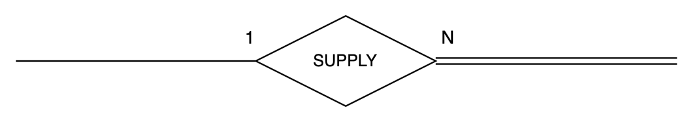
\includegraphics[width=0.7\textwidth]{images/relationships/supply.png}
  \caption{\textit{Supply Relationship}}
\end{figure}

The "Supply" relationship is between the Supplier and the Product. A supplier can supply multiple products. It tracks the quantity, date, and price of supplied products.

\subsubsection{Supervision}
\begin{figure}[H]
  \centering
  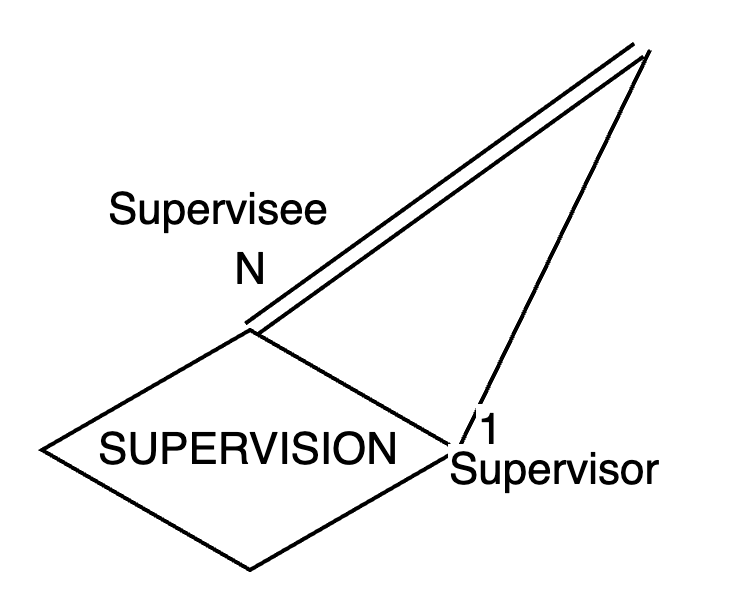
\includegraphics[width=0.7\textwidth]{images/relationships/supervision.png}
  \caption{\textit{Supervision Relationship}}
\end{figure}

The "Supervision" relationship is a recursive relationship among Employees. An employee can supervise others, ensuring a clear management hierarchy.

\subsubsection{Wishlist}
\begin{figure}[H]
  \centering
  
\includegraphics[width=0.7\textwidth]{images/relationships/wishlist.png}
  \caption{\textit{Wishlist Relationship}}
\end{figure}

The "Wishlist" relationship is between the customer and the product. A wishlist must be created by a customer. However, a wishlist can be empty, or it can include several products. It takes as an attribute the total amount (price) of the products. This relationship ensures that the customer can save the items he/she wishes to obtain later on.

\subsubsection{Works For}
\begin{figure}[H]
  \centering
  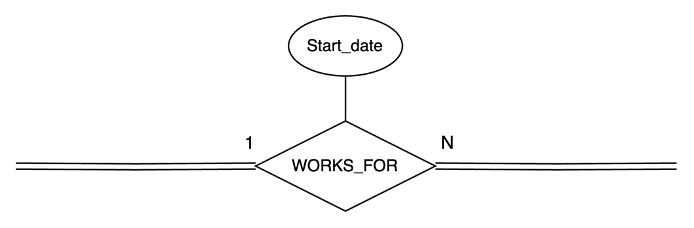
\includegraphics[width=0.7\textwidth]{images/relationships/works_for.png}
  \caption{\textit{Works For Relationship}}
\end{figure}

The "Works For" relationship connects the Employee and the Department. Many employees work for one department, and each department must have at least one employee.

\subsubsection{Works In}
\begin{figure}[H]
  \centering
  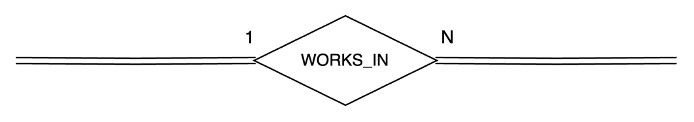
\includegraphics[width=0.7\textwidth]{images/relationships/works_in.png}
  \caption{\textit{Works In Relationship}}
\end{figure}

The "Works In" relationship links the Employee and the Branch. A branch must have at least one employee, and each employee works in one branch.
\section{ER to Relational Mapping}

\subsection{Mapping of Strong Entity Types}

\begin{itemize}
  \item For each regular (strong) entity type E in the ER schema, create a relation R that includes all the simple (atomic) attributes of E.
  \item Choose one of the key attributes of E as the primary key for R.
  \item If the chosen key of E is composite, the set of simple attributes that form it will together form the primary key of the relation R. \cite{slides}
\end{itemize}

\subsubsection{Branch}

Branch (\underline{Phone\_number}, Name, Country, State, City, Street, Building, Apartment)

We created the relation Branch including various attributes of the strong entity Branch. We included all the simple (atomic) attributes of Branch that are Name and Phone\_number. Moreover, we decomposed the composite attribute Address into simple attributes as country, state, city, street, building , and apartment. Furthermore, we didn't include the composite multi-valued attribute which is Work\_hours as we'll create its own relation later. Finally, we chose the key attribute Phone\_number to be the primary key that uniquely identifies the relation Branch.

\subsubsection{Category}

Category (\underline{Name}, Description)

We created the relation Category including the two atomic attributes of the strong entity Category that are Name and Description. Additionally, we chose the key attribute Name as the primary key.

\subsubsection{Coupon}

Coupon (\underline{Code}, Description, Discount\_percent, Times\_used, Minimum\_order\_amount,\\
Maximum\_order\_amount, Usage\_limit, Valid\_from, Valid\_to)

We created the relation Coupon including attributes of the strong entity Coupon. We included all atomic attributes which are Code, Description, Discount\_percent, Times\_used, Minimum\_order\_amount, Maximum\_order\_amount, and Usage\_limit. Furthermore, we decomposed the composite attribute Valid into two simple attributes which are Valid\_from and Valid\_to. Finally, we chose the key attribute Code as a primary key.

\subsubsection{Customer}

Customer (\underline{Phone\_number}, Email, First\_name, Last\_name, Gender, Registration\_date, Password\_hashed, Date\_of\_birth, Country, State, City, Street, Building, Apartment)

We created the relation Customer including different attributes of the strong entity Customer. We included all the atomic attribute which are Phone\_number, Email, Gender, Registration\_date, Password\_hashed and Date\_of\_birth. Moreover, we decomposed the two composite attribute Name and Address as First\_name and Last\_name and Country, State, City, Street, Building and Apartment, respectively.

\subsubsection{Department}

Department (\underline{Name}, Number\_of\_employees)

We created the relation Department including various attributes of the strong entity Department. We included all the simple attributes which are Name and Number\_of\_employees, such that Name acts a primary key and Number\_of\_employees as a derived attribute. Furthermore, we didn't include the multi-valued attribute which is Locations as we'll create its own relation later.


\subsubsection{Driver}

Driver (\underline{License\_number}, Driving\_experience\_years, License\_expiry\_date)

We created the relation Driver including all the atomic attributes of the strong entity Driver which are: the key attribute which is License\_number as a primary key, Driving\_experience\_years and License\_expiry\_date.

\subsubsection{Employee}

Employee (\underline{SSN}, Position, Salary, Hire\_date, Gender, Date\_of\_birth, Email, First\_name, Last\_name, \\
Phone\_number, Country, State, City, Street, Building, Apartment)

We created the relation Employee including various attributes of the regular entity Employee. We included all the simple attributes which are: SSN, Position, Salary, Hire\_date, Gender, Date\_of\_birth, Email and Phone\_number. Moreover, we decomposed the two composite attribute Name and Address as First\_name and Last\_name and Country, State, City, Street, Building and Apartment, respectively. Finally, we chose the key attribute SSN as the primary key.

\subsubsection{Order}

Order (\underline{Order\_id}, Notes, Payment\_method, Total\_amount, Is\_online)

We created the relation Order including all the atomic attributes of the strong entity Order which are: the key attribute which is Order\_id as a primary key, Notes, Payment\_method, Total\_amount and Is\_online.

\subsubsection{Product}

Product (\underline{SKU}, Name, Price, Description, Weight, Brand, Width, Height, Length)

We created the relation Product including various attributes of the regular entity Product. We included all the simple attributes which are SKU, Name, Price, Description, Weight and Brand. Moreover, we decomposed the composite attribute Dimensions into three atomic attributes which are: Width, Height and Length. Furthermore, we didn't include the multi-valued attributes which are Image\_URLs and Colors as we'll create relations from them later. Finally, we chose the key attribute SKU as the primary key.

\subsubsection{Supplier}

Supplier (\underline{Website}, Supplier\_name, Contact\_person\_email, \\
Contact\_person\_first\_name, Contact\_person\_last\_name, Contact\_person\_phone\_number )

We created the relation Supplier including various attributes of the regular entity Supplier. We included all the simple attributes which are: Supplier\_name and Website. Moreover, we decomposed the composite attribute into two atomic attributes and a composite attribute, which are Email and Phone\_number and Name, respectively. Furthermore, we decomposed Name into two atomic attributes which are First\_name and Last\_name. Finally, we chose the key attribute Website as the primary key.

\subsubsection{Support Ticket}

Support\_Ticket (\underline{Ticket\_id}, Description, Subject, Status, Priority)

We created the relation Support\_Ticket including attributes of the regular entity Support\_Ticket. We included all the simple attributes which are: Ticket\_id, Description, Subject, Status and Priority.  Finally, we chose the key attribute Ticket\_id as the primary key.

\subsection{Mapping of Weak Entity Types}

\begin{itemize}
  \item	According to Elmasri and Navathe, in Fundamentals of Database Systems (2015), "For each weak entity type W in the ER schema with owner entity type E, create a relation R \& include all simple attributes (or simple components of composite attributes) of W as attributes of R.
  \item	Also, include as foreign key attributes of R the primary key attribute(s) of the relation(s) that correspond to the owner entity type(s).
  \item	The primary key of R is the combination of the primary key(s) of the owner(s) and the partial key of the weak entity type W, if any." \cite{elmasri}
\end{itemize}

\subsubsection{Dependent}

Dependent (\underline{\textit{Employee\_SSN}}, \underline{Name}, Gender, Date\_of\_birth, Relationship)

We created a relation Dependent for the weak entity type Dependent with employee entity type Employee. We included all the atomic attributes of Dependent which are Name, Gender, Date\_of\_birth, and Relationship. Moreover, we created the foreign key Employee\_SSN which references to the primary key of Employee which is SSN. Finally, we assigned the tuple Employee\_SSN and the weak attribute Name as the primary key of this relation.

\subsection{Mapping of Binary 1:1 Relationship Types}

\begin{itemize}
  \item According to Elmasri and Navathe, in Fundamentals of Database Systems (2015), "For each binary 1:1 relationship type R in the ER schema, identify the relations S and T that correspond to the entity types participating in R.
  \item Foreign Key approach: Choose one of the relations-say S-and include a foreign key in S the primary key of T. It is better to choose an entity type with total participation in R in the role of S." \cite{elmasri}
\end{itemize}

\subsubsection{Redeem}

Coupon (\underline{Code}, Description, Discount\_percent, Times\_used, Minimum\_order\_amount, \\
Maximum\_order\_amount, Usage\_limit, Valid\_from, Valid\_to, \textit{Order\_ID}, \\
Discount\_amount\_ Redeem\_date)

The 1:1 relationship Redeem is mapped by choosing the participating entity type Coupon to serve in the role of S, because both participating entity types have a partial participation in the Redeem relationship type, so, it doesn't matter which one we choose. Moreover, we chose Order\_ID as the foreign key referencing to the primary key of Order. Finally, we added all the atomic attributes of the relationship Redeem to the relation Coupon.

\subsubsection{Manages Branch}

Branch (\underline{Phone\_number}, Name, Country, State, City, Street, Building, Apartment, \textit{Employee\_SSN})

The 1:1 relationship Manages\_branch is mapped by choosing the participating entity type Branch to serve in the role of S, because its participation in the Manages\_branch relationship type is total. Moreover, we added the foreign key Employee\_SSN referencing to the primary key of Employee.

\subsubsection{Is Driver}

Driver (\underline{License\_number}, Driving\_experience\_years, License\_expiry\_date, \textit{Employee\_SSN})

The 1:1 relationship Is\_driver is mapped by choosing the participating entity type Driver to serve in the role of S, because its participation in the Is\_driver relationship type is total. Moreover, we add the foreign key Employee\_SSN referencing to the primary key of Employee.

\subsubsection{Manages Department}

Department(\underline{Name}, Number\_of\_employees, \textit{Employee\_SSN}, Manager\_start\_date)

The 1:1 relationship Manages\_department is mapped by choosing the participating entity type Department to serve in the role of S, because its participation in the Manages\_department relationship type is total. Moreover, we add the foreign key Employee\_SSN referencing to the primary key of Employee. Finally, we added the atomic attribute of the relationship Manages\_department to the relation Coupon.

\subsection{Mapping of Binary 1:N Relationship Types}

\begin{itemize}
  \item According to Elmasri and Navathe, in Fundamentals of Database Systems (2015), "For each regular binary 1:N relationship type R, identify the relation S that represent the participating entity type at the N-side of the relationship type.
  \item Include as foreign key in S the primary key of the relation T that represents the other entity type participating in R.
  \item Include any simple attributes of the 1:N relation type as attributes of S." \cite{elmasri}
\end{itemize}

\subsubsection{Subcategory}

Category (\underline{Name}, Description, \textit{Parent\_Category\_Name})

The 1:N relationship Subcategory is mapped by choosing the participating entity type Category to serve in the role of S, because it is a self-relationship. Moreover, we added the foreign key Parent\_Category\_Name to connect the entity type to itself.

\subsubsection{Contains}

Product (\underline{SKU}, Name, Price, Description, Weight, Brand, Width, Height, Length, \textit{Category\_name})

The 1:N relationship Contains is mapped by choosing the participating entity type Product to serve in the role of S, because its participation in the Contains relationship is from the N-side. Moreover, we added the foreign key Category\_name to connect the two participating entities.

\subsubsection{Supply}

Product (\underline{SKU}, Name, Price, Description, Weight, Brand, Width, Height, Length, \textit{Category\_name}, \\
\textit{Supplier\_website})

The 1:N relationship Supply is mapped by choosing the participating entity type Product to serve in the role of S, because its participation in the Supply relationship is from the N-side. Moreover, we added the foreign key Supplier\_website to connect the two participating entities.

\subsubsection{Works In}

Employee (\underline{SSN}, Position, Salary, Hire\_date, Gender, Date\_of\_birth, Email, First\_name, Last\_name,\\
Phone\_number, Country, State, City, Street, Building, Apartment, \textit{Branch\_phone\_number})

The 1:N relationship Works\_in is mapped by choosing the participating entity type Employee to serve in the role of S, because its participation in the Works\_in relationship is from the N-side. Moreover, we added the foreign key Branch\_phone\_number to connect the two participating entities.

\subsubsection{Supervision}

Employee (\underline{SSN}, Position, Salary, Hire\_date, Gender, Date\_of\_birth, Email, First\_name, \\
Last\_name, Phone\_number, Country, State, City, Street, Building, Apartment, \textit{Branch\_phone\_number}, \\
\textit{Supervisor\_SSN})

The 1:N relationship Supervision is mapped by choosing the participating entity type Employee to serve in the role of S, because it is a self-relationship. Moreover, we added the foreign key Supervisor\_SSN to connect the entity type to itself.

\subsubsection{Physical Checkout}

Order (\underline{Order\_id}, Notes, Payment\_method, Total\_amount, Is\_online, \textit{Employee\_SSN})

The 1:N relationship Physical\_checkout is mapped by choosing the participating entity type Order to serve in the role of S, because its participation in the Physical\_checkout relationship is from the N-side. Moreover, we added the foreign key Employee\_SSN to connect the two participating entities.

\subsubsection{Made By}

Order (\underline{Order\_id}, Notes, Payment\_method, Total\_amount, Is\_online, \textit{Employee\_SSN}, \\
\textit{Customer\_phone\_number}, Date)

The 1:N relationship Made\_by is mapped by choosing the participating entity type Order to serve in the role of S, because its participation in the Made\_by relationship is from the N-side. Moreover, we added the foreign key Customer\_phone\_number to connect the two participating entities. Finally, we added the atomic attribute of the relationship Made\_by to the relation Order.

\subsubsection{Works For}

Employee (\underline{SSN}, Position, Salary, Hire\_date, Gender, Date\_of\_birth, Email, First\_name, Last\_name, \\
Phone\_number, Country, State, City, Street, Building, Apartment, \textit{Branch\_phone\_number}, \\
\textit{Supervisor\_SSN}, \textit{Department\_name})

The 1:N relationship Works\_for is mapped by choosing the participating entity type Employee to serve in the role of S, because its participation in the Works\_for relationship is from the N-side. Moreover, we added the foreign key Department\_name to connect the two participating entities. Finally, we added all the atomic attributes of the relationship Works\_for to the relation Employee.

\subsubsection{Dependents Of}

Dependent (Owner\_SSN, Name, Gender, Date\_of\_birth, Relationship, \textit{Employee\_SSN})

The 1:N relationship Dependents\_of is mapped by choosing the participating entity type Dependent to serve in the role of S, because its participation in the Dependents\_of relationship is from the N-side. Moreover, we added the foreign key Employee\_SSN to connect the two participating entities.

\subsubsection{Assigned To}

Support\_ticket (\underline{Ticket\_id}, Description, Subject, Status, Priority, \textit{Employee\_SSN})

The 1:N relationship Assigned\_to is mapped by choosing the participating entity type Support\_ticket to serve in the role of S, because its participation in the Assigned\_to relationship is from the N-side. Moreover, we added the foreign key Employee\_SSN to connect the two participating entities.

\subsubsection{Delivers}

Order (\underline{Order\_id}, Notes, Payment\_method, Total\_amount, Is\_online, \textit{Employee\_SSN}, \\
\textit{Customer\_phone\_number}, Date, \textit{Driver\_license\_number})

The 1:N relationship Delivers is mapped by choosing the participating entity type Order to serve in the role of S, because its participation in the Delivers relationship is from the N-side. Moreover, we added the foreign key Driver\_license\_number to connect the two participating entities.

\subsubsection{Requests}

Support\_ticket (\underline{Ticket\_id}, Description, Subject, Status, Priority, \textit{Employee\_SSN}, \\
\textit{Customer\_phone\_number})

The 1:N relationship Requests is mapped by choosing the participating entity type Support\_ticket to serve in the role of S, because its participation in the Requests relationship is from the N-side. Moreover, we added the foreign key Custom\_phone\_number to connect the two participating entities.

\subsection{Mapping of Multivalued Attributes}

\begin{itemize}
  \item According to Elmasri and Navathe, in Fundamentals of Database Systems (2015), "For each regular binary M:N relationship type R, create a new relation S to represent R.
  \item Include as foreign key attributes in S the primary keys of the relations that represent the participating entity types; combination will form the primary key of S.
  \item Also include any simple attributes of the M:N relationship type (or simple components of composite attributes) as attributes of S." \cite{elmasri}
\end{itemize}

\subsubsection{Wishlist}

Wishlist (\underline{SKU}, \underline{\textit{Customer\_phone\_number}}, Total\_amount)

The M:N relationship Wishlist from the ER diagram is mapped by creating a relation Wishlist in the relational database schema. The primary keys of the Product and Customer relations are included as foreign keys in Wishlist and renamed Product\_SKU and Customer\_phone\_number, respectively. The attribute Total\_amount represents the total amount of the product in the wish list. The primary key of Wishlist is the tuple of foreign keys \{Product\_SKU, Customer\_phone\_number\}.

\subsubsection{Located In}

Located\_in (\underline{\textit{Product\_SKU}}, \underline{\textit{Branch\_phone\_number}}, Quantity, Shelf\_location)

The M:N relationship type Located\_in from the ER diagram is mapped by creating a relation Located\_in in the relational database schema. The primary keys of the Product and Branch relations are included as foreign keys in Located\_in and renamed Product\_SKU and Branch\_phone\_number, respectively. Attributes Quantity and Shelf\_location in Located\_in represent the Quantity and Shelf\_location attributes of the relation type. The primary key of the Located\_in relation is the combination of the foreign key attributes \{Product\_SKU, Branch\_phone\_number\}.

\subsubsection{Reviews}

Reviews (\underline{\textit{Product\_SKU}}, \underline{\textit{Customer\_phone\_number}}, Review\_date, Rating, Comment, Description)

The M:N relationship type Reviews from the ER diagram is mapped by creating a relation Reviews in the relational database schema. The primary keys of the Product and Customer relations are included as foreign keys in Reviews and renamed Product\_SKU and Customer\_phone\_number, respectively. Attributes Review\_date, Rating, Comment, and Description in Reviews represent the corresponding attributes of the relation type. The primary key of the Reviews relation is the combination of the foreign key attributes \{Product\_SKU, Customer\_phone\_number\}. Furthermore, we didn't include the multi-valued attribute Image\_URLs as we'll create its own relation later.

\subsubsection{Purchased}

Purchased (\underline{\textit{Product\_SKU}}, \underline{\textit{Order\_id}}, Quantity, Amount)

The M:N relationship type Purchased from the ER diagram is mapped by creating a relation Purchased in the relational database schema. The primary keys of the Product and Order relations are included as foreign keys in Purchased and renamed Product\_SKU and Order\_id, respectively. Attributes Quantity and Amount in Purchased represent the corresponding attributes of the relation type. The primary key of the Purchased relation is the combination of the foreign key attributes \{Product\_SKU, Order\_id\}.

\subsection{Mapping of Binary M:N Relationship Types}

\begin{itemize}
  \item According to Elmasri and Navathe, in Fundamentals of Database Systems (2015), "For each multivalued attribute A, create a new relation R.
  \item This relation R will include an attribute corresponding to A, plus the primary key attribute K-as a foreign key in R-of the relation that represents the entity type of relationship type that has A as an attribute.
  \item The primary key of R is the combination of A and K. If the multivalued attribute is composite, we include its simple components." \cite{elmasri}
\end{itemize}

\subsubsection{Colors}

Colors (\underline{\textit{Product\_SKU}}, \underline{Product\_color})

The relation Colors is created. The attribute Product\_color represents the multivalued attribute Colors of Product, while Product\_SKU—as foreign key—represents the primary key of the Product relation. The primary key of Color\_s is the combination of \{Product\_SKU, Product\_color\}.

\subsubsection{Image URLs}

Image\_URLs (\underline{\textit{Product\_SKU}}, \textit{Customer\_phone\_number}, \underline{Product\_Image\_URL})

The relation Image\_URLs is created. The attribute Product\_Image\_URL represents the multivalued attribute Image\_URL of Product, while Product\_SKU—as foreign key—represents the primary key of the Product relation. The primary key of Image\_URLs is the combination of \{Product\_SKU, Product\_Image\_URL\}.

\subsubsection{Working Hours}

Working\_hours (\underline{\textit{Branch\_phone\_number}}, \underline{Day}, \underline{Opening\_hour}, \underline{Closing\_hour})

The relation Working\_hours is created. The attributes Day, Opening\_hour, and Closing\_hour represent the composite-multivalued attribute Work\_hours of Branch, while Branch\_phone\_number—as foreign key—represents the primary key of the Branch relation. The primary key of Working\_hours is the combination of \{Branch\_phone\_number, Day, Opening\_hour, Closing\_hour\}.

\subsubsection{Department Location}

Department\_location (\underline{Department\_name}, \underline{Location})

The relation Department\_location is created. The attribute Location represents the multivalued attribute Locations of Department, while Department\_name—as foreign key—represents the primary key of the Department relation. The primary key of Department\_location is the combination of \\
\{Department\_name, Location\}.

\section{Final Display -- All Tables}

\Table{Branch Table}{\underline{Phone\_number} & Name & Country & State & City & Street & Building & Apartment & \textit{Employee\_SSN}}

\Table{Category Table}{\underline{Name} & Description & \textit{Parent\_Category\_Name}}

\Table{Colors Table}{\underline{\textit{Product\_SKU}} & \underline{Product\_color}}

\TableWide{Coupon Table}{\underline{Code} & Description & Discount\_percent & Times\_used & Minimum\_order\_amount & Maximum\_order\_amount & Usage\_limit & Valid\_from & Valid\_to & \textit{Order\_ID} & Discount\_amount & Redeem\_date}

\TableWide{Customer Table}{\underline{Phone\_number} & Email & First\_name & Last\_name & Gender & Registration\_date & Password\_hashed & Date\_of\_birth & Country & State & City & Street & Building & Apartment}

\Table{Department Table}{\underline{Name} & Number\_of\_employees & \textit{Employee\_SSN} & Manager\_start\_date}

\Table{Department Location Table}{\underline{Department\_name} & \underline{Location}}

\Table{Dependent Table}{\underline{\textit{Employee\_SSN}} & \underline{Name} & Gender & Date\_of\_birth & Relationship}

\Table{Driver Table}{\underline{License\_number} & Driving\_experience\_years & License\_expiry\_date & \textit{Employee\_SSN}}

\TableWide{Employee Table}{\underline{SSN} & Position & Salary & Hire\_date & Gender & Date\_of\_birth & Email & First\_name & Last\_name & Phone\_number & Country & State & City & Street & Building & Apartment & \textit{Branch\_phone\_number} & \textit{Supervisor\_SSN} & \textit{Department\_name}}

\Table{Image URLs Table}{\underline{\textit{Product\_SKU}} & \textit{Customer\_phone\_number} & \underline{Product\_Image\_URL}}

\Table{Located In Table}{\underline{\textit{Product\_SKU}} & \underline{\textit{Branch\_phone\_number}} & Quantity & Shelf\_location}

\TableWide{Order Table}{\underline{Order\_id} & Notes & Payment\_method & Total\_amount & Is\_online & \textit{Employee\_SSN} & \textit{Customer\_phone\_number} & Date & \textit{Driver\_license\_number}}

\TableWide{Product Table}{\underline{SKU} & Name & Price & Description & Weight & Brand & Width & Height & Length & \textit{Category\_name} & \textit{Supplier\_website}}

\Table{Purchased Table}{\underline{\textit{Product\_SKU}} & \underline{\textit{Order\_id}} & Quantity & Amount}

\Table{Reviews Table}{\underline{\textit{Product\_SKU}} & \underline{\textit{Customer\_phone\_number}} & Review\_date & Rating & Comment & Description}

\Table{Support Ticket Table}{\underline{Ticket\_id} & Description & Subject & Status & Priority & \textit{Employee\_SSN} & \textit{Customer\_phone\_number}}

\TableWide{Supplier Table}{\underline{Website} & Supplier\_name & Contact\_person\_email & Contact\_person\_first\_name & Contact\_person\_last\_name & Contact\_person\_phone\_number}

\Table{Wishlist Table}{\underline{SKU} & \underline{\textit{Customer\_phone\_number}} & Total\_amount}

\Table{Working Hours Table}{\underline{\textit{Branch\_phone\_number}} & \underline{Day} & \underline{Opening\_hour} & \underline{Closing\_hour}}

\section{Tables' States}

\TableWide{Branch}{
  \underline{Phone\_number} & Name & Country & State & City & Street & Building & Apartment & \textit{Employee\_SSN} \\
  \hline
  +96111111111 & Beirut Main & Lebanon & Beirut & Beirut & Hamra & 10 & 1 & 123456789 \\
  +96122222222 & Tripoli Branch & Lebanon & North & Tripoli & Mina Street & 5 & 12 & 987654321 \\
  +96133333333 & Sidon Hub & Lebanon & South & Sidon & Corniche & 3 & 6 & 543216789 \\
  +96144444444 & Zahle Branch & Lebanon & Beqaa & Zahle & Bekaa St & 8 & 4 & 123459876 \\
  +96155555555 & Jounieh Store & Lebanon & Mount Lebanon & Jounieh & Coastal Rd & 7 & 3 & 567894321 \\
  +96166666666 & Byblos Outlet & Lebanon & Mount Lebanon & Byblos & Roman Street & 6 & 5 & 678912345 \\
  +96177777777 & Tyre Shop & Lebanon & South & Tyre & Port Road & 2 & 1 & 876543219 \\
  +96188888888 & Baalbek Point & Lebanon & Beqaa & Baalbek & Temple Rd & 4 & 2 & 345678912 \\
  +96199999999 & Batroun Corner & Lebanon & North & Batroun & Old City & 1 & 1 & 456789123 \\
  +96112345678 & Downtown Center & Lebanon & Beirut & Beirut & Downtown & 5 & 11 & 234567891 \\
  +96198765432 & Achrafieh Depot & Lebanon & Beirut & Achrafieh & Armenia St & 9 & 8 & 234567891 \\
  +96124681357 & Dora Warehouse & Lebanon & Mount Lebanon & Dora & Industrial Zone & 3 & 2 & 789123456 \\
  +96165432198 & Aley Branch & Lebanon & Mount Lebanon & Aley & Souk Street & 4 & 10 & 654321987 \\
  +96111223344 & Choueifat Station & Lebanon & Mount Lebanon & Choueifat & Railway Rd & 2 & 7 & 321987654 \\
  +96144332211 & Antelias Spot & Lebanon & Mount Lebanon & Antelias & Highway Rd & 8 & 5 & 987123456
}

\Table{Category}{
  \underline{Name} & Description & \textit{Parent\_Category\_Name} \\
  \hline
  Electronics & Devices and gadgets & NULL \\
  Clothing & Apparel and fashion items & NULL \\
  Furniture & Home and office furniture & NULL \\
  Books & Printed and digital books & Stationery \\
  Groceries & Food and daily supplies & Health \\
  Sports & Sporting equipment and apparel & Clothing \\
  Beauty & Cosmetics and skincare products & Health \\
  Toys & Toys for kids and adults & Sports \\
  Automotive & Car parts and accessories & Electronics \\
  Jewelry & Watches, rings, and necklaces & Fashion \\
  Health & Medical supplies and equipment & Beauty \\
  Stationery & Office and school supplies & Furniture \\
  Pets & Pet food and accessories & Groceries \\
  Music & Instruments and music equipment & Art \\
  Art & Art supplies and crafts & Stationery
}

\Table{Colors}{
  \underline{\textit{Product\_SKU}} & \underline{Product\_color} \\
  \hline
  1001 & Red \\
  1002 & Blue \\
  1003 & Green \\
  1004 & Black \\
  1005 & White \\
  1006 & Yellow \\
  1007 & Pink \\
  1008 & Purple \\
  1009 & Orange \\
  1010 & Brown \\
  1011 & Gray \\
  1012 & Gold \\
  1013 & Silver \\
  1014 & Beige \\
  1015 & Navy
}

\TableWide{Coupon}{
  \underline{Code} & Description & Discount\_percent & Times\_used & Minimum\_order\_amount & Maximum\_order\_amount & Usage\_limit & Valid\_from & Valid\_to & \textit{Order\_ID} & Discount\_amount & Redeem\_date \\
  \hline
  DIS10 & 10\% off & 10 & 25 & 50 & 500 & 100 & 2024-01-01 & 2024-12-31 & O101 & 5 & 2024-10-01 \\
  DIS20 & 20\% off & 20 & 40 & 100 & 1000 & 50 & 2024-02-01 & 2024-11-30 & O102 & 10 & 2024-09-15 \\
  FREESHIP & Free shipping & 0 & 100 & 0 & 200 & 200 & 2024-05-01 & 2024-10-31 & O103 & 0 & 2024-08-12 \\
  SAVE15 & 15\% off & 15 & 60 & 75 & 750 & 75 & 2024-03-01 & 2024-09-30 & O104 & 12 & 2024-07-07 \\
  BOGO & Buy 1 Get 1 & 50 & 20 & 100 & 1000 & 25 & 2024-01-01 & 2024-08-31 & O105 & 50 & 2024-06-06 \\
  HOLIDAY50 & 50\% off & 50 & 10 & 200 & 2000 & 10 & 2024-12-01 & 2024-12-31 & O106 & 100 & 2024-12-05 \\
  FLASH5 & 5\% off & 5 & 150 & 25 & 250 & 500 & 2024-07-01 & 2024-08-01 & O107 & 2 & 2024-07-12 \\
  SUMMER30 & 30\% off & 30 & 80 & 150 & 1500 & 30 & 2024-06-01 & 2024-09-01 & O108 & 45 & 2024-07-20 \\
  BLACKFRIDAY & 40\% off & 40 & 90 & 300 & 3000 & 100 & 2024-11-29 & 2024-11-29 & O109 & 120 & 2024-11-29 \\
  NEWYEAR25 & 25\% off & 25 & 70 & 200 & 2000 & 75 & 2024-12-31 & 2025-01-01 & O110 & 50 & 2024-12-31 \\
  WELCOME & 10\% for new users & 10 & 200 & 50 & 500 & 300 & 2024-01-01 & 2024-12-31 & O111 & 10 & 2024-01-10 \\
  VIP20 & 20\% VIP discount & 20 & 30 & 150 & 1500 & 50 & 2024-01-01 & 2024-12-31 & O112 & 30 & 2024-02-14 \\
  BIRTHDAY & 25\% off on birthday & 25 & 10 & 100 & 1000 & 20 & 2024-01-01 & 2024-12-31 & O113 & 25 & 2024-03-03 \\
  CLEARANCE & Up to 70\% off & 70 & 5 & 500 & 5000 & 10 & 2024-11-01 & 2024-11-15 & O114 & 350 & 2024-11-05 \\
  LOYALTY & 15\% off for loyal customers & 15 & 50 & 100 & 1000 & 60 & 2024-01-01 & 2024-12-31 & O115 & 15 & 2024-04-22
}

\TableWide{Customer}{
  \underline{Phone\_number} & Email & First\_name & Last\_name & Gender & Registration\_date & Password\_hashed & Date\_of\_birth & Country & State & City & Street & Building & Apartment \\
  \hline
  +96134567890 & john.doe@gmail.com & John & Doe & Male & 2023-02-14 & ******** & 1990-03-05 & Lebanon & Beirut & Beirut & Hamra & 12 & 2 \\
  +96198765432 & jane.smith@yahoo.com & Jane & Smith & Female & 2022-10-22 & ******** & 1985-06-15 & Lebanon & North & Tripoli & Mina Street & 4 & 5 \\
  +96145678901 & alice.brown@outlook.com & Alice & Brown & Female & 2024-03-01 & ******** & 1992-01-20 & Lebanon & South & Sidon & Corniche & 7 & 3 \\
  +96167890123 & bob.jones@hotmail.com & Bob & Jones & Male & 2021-07-18 & ******** & 1988-11-02 & Lebanon & Mount Lebanon & Jounieh & Coastal Rd & 8 & 6 \\
  +96178901234 & charlie.evans@gmail.com & Charlie & Evans & Male & 2020-05-30 & ******** & 1995-09-09 & Lebanon & Beirut & Achrafieh & Armenia St & 9 & 7 \\
  +96189012345 & diana.lee@aol.com & Diana & Lee & Female & 2023-01-15 & ******** & 1989-04-25 & Lebanon & Beqaa & Zahle & Bekaa St & 2 & 1 \\
  +96190123456 & frank.wilson@protonmail.com & Frank & Wilson & Male & 2019-11-20 & ******** & 1975-12-12 & Lebanon & North & Batroun & Old City & 1 & 1 \\
  +96101234567 & emma.white@gmail.com & Emma & White & Female & 2024-06-01 & ******** & 1993-08-17 & Lebanon & Mount Lebanon & Byblos & Roman Street & 6 & 3 \\
  +96123456789 & george.king@live.com & George & King & Male & 2022-09-05 & ******** & 1980-02-22 & Lebanon & South & Tyre & Port Road & 5 & 10 \\
  +96156789012 & hannah.scott@gmail.com & Hannah & Scott & Female & 2021-12-25 & ******** & 2000-07-30 & Lebanon & Mount Lebanon & Antelias & Highway Rd & 8 & 9 \\
  +96167890124 & jack.miller@yahoo.com & Jack & Miller & Male & 2023-08-10 & ******** & 1987-05-15 & Lebanon & Beqaa & Baalbek & Temple Rd & 4 & 2 \\
  +96178901235 & isabella.taylor@outlook.com & Isabella & Taylor & Female & 2024-02-02 & ******** & 1991-03-18 & Lebanon & Beirut & Downtown & Downtown & 3 & 11 \\
  +96189012346 & kevin.martin@hotmail.com & Kevin & Martin & Male & 2022-07-19 & ******** & 1984-09-25 & Lebanon & Mount Lebanon & Aley & Souk Street & 4 & 10 \\
  +96190123457 & laura.harris@icloud.com & Laura & Harris & Female & 2021-04-22 & ******** & 1996-11-05 & Lebanon & Beirut & Hamra & Hamra St & 2 & 8 \\
  +96101234568 & mike.anderson@protonmail.com & Mike & Anderson & Male & 2023-05-03 & ******** & 1998-01-11 & Lebanon & Mount Lebanon & Choueifat & Railway Rd & 7 & 3
}

\TableWide{Department}{
  \underline{Name} & Number\_of\_employees & \textit{Employee\_SSN} & Manager\_start\_date \\
  \hline
  Sales & 30 & 123456789 & 2022-03-01 \\
  Marketing & 25 & 987654321 & 2021-06-15 \\
  HR & 15 & 123459876 & 2023-01-10 \\
  Finance & 20 & 567894321 & 2019-10-05 \\
  Operations & 35 & 543216789 & 2020-08-25 \\
  IT & 10 & 678912345 & 2024-04-18 \\
  Customer Support & 12 & 876543219 & 2022-09-12 \\
  Logistics & 18 & 345678912 & 2020-11-20 \\
  Legal & 8 & 456789123 & 2021-02-14 \\
  R\&D & 14 & 234567891 & 2018-12-22 \\
  Training & 9 & 789123456 & 2023-03-27 \\
  Procurement & 11 & 654321987 & 2021-05-30 \\
  Admin & 7 & 321987654 & 2022-07-04 \\
  Facilities & 6 & 987123456 & 2019-06-01 \\
  Compliance & 5 & 654789321 & 2020-01-17
}

\Table{Department location}{
  \underline{Department\_name} & \underline{Location} \\
  \hline
  Sales & Beirut \\
  Marketing & Tripoli \\
  HR & Zahle \\
  Finance & Jounieh \\
  Operations & Sidon \\
  IT & Byblos \\
  Customer Support & Tyre \\
  Logistics & Baalbek \\
  Legal & Batroun \\
  R\&D & Achrafieh \\
  Training & Dora \\
  Procurement & Aley \\
  Admin & Choueifat \\
  Facilities & Antelias \\
  Compliance & Downtown Beirut
}

\Table{Dependent}{
  \underline{\textit{Employee\_SSN}} & \underline{Name} & Gender & Date\_of\_birth & Relationship \\
  \hline
  123456789 & Sarah Doe & Female & 2015-04-15 & Daughter \\
  987654321 & James Smith & Male & 2013-07-20 & Son \\
  123459876 & Emily Brown & Female & 2017-02-28 & Daughter \\
  567894321 & Lucas Jones & Male & 2018-11-05 & Son \\
  543216789 & Olivia Evans & Female & 2016-09-12 & Daughter \\
  678912345 & Ethan White & Male & 2020-03-22 & Son \\
  876543219 & Chloe Lee & Female & 2014-08-01 & Daughter \\
  345678912 & Liam Harris & Male & 2015-12-15 & Son \\
  456789123 & Mia Taylor & Female & 2018-10-03 & Daughter \\
  234567891 & Noah Wilson & Male & 2021-06-08 & Son \\
  789123456 & Sophia Martin & Female & 2019-05-25 & Daughter \\
  654321987 & Benjamin Scott & Male & 2012-01-19 & Son \\
  321987654 & Emma Anderson & Female & 2015-07-13 & Daughter \\
  987123456 & Mason Miller & Male & 2018-03-09 & Son \\
  654789321 & Ava Thomas & Female & 2016-02-04 & Daughter
}

\Table{Driver}{
  \underline{License\_number} & Driving\_experience\_years & License\_expiry\_date & \textit{Employee\_SSN} \\
  \hline
  DL1001 & 5 & 2025-12-31 & 123456789 \\
  DL1002 & 3 & 2026-06-30 & 987654321 \\
  DL1003 & 10 & 2027-04-15 & 567894321 \\
  DL1004 & 7 & 2028-01-10 & 543216789 \\
  DL1005 & 2 & 2026-08-20 & 678912345 \\
  DL1006 & 6 & 2024-11-25 & 876543219 \\
  DL1007 & 8 & 2029-09-09 & 345678912 \\
  DL1008 & 12 & 2025-05-05 & 456789123 \\
  DL1009 & 4 & 2024-07-18 & 234567891 \\
  DL1010 & 15 & 2030-03-30 & 789123456 \\
  DL1011 & 1 & 2024-12-15 & 654321987 \\
  DL1012 & 9 & 2027-02-14 & 321987654 \\
  DL1013 & 14 & 2031-06-11 & 987123456 \\
  DL1014 & 11 & 2029-12-21 & 654789321 \\
  DL1015 & 13 & 2026-10-07 & 123459876
}

\TableWide{Employee}{
  \underline{SSN} & Position & Salary & Hire\_date & Gender & Date\_of\_birth & Email & First\_name & Last\_name & Phone\_number & Country & State & City & Street & Building & Apartment & \textit{Branch\_phone\_number} & \textit{Supervisor\_SSN} & \textit{Department\_name} \\
  \hline
  123456789 & Manager & 3000 & 2022-03-01 & Male & 1985-05-12 & john.doe@example.com & John & Doe & +96134567890 & Lebanon & Beirut & Beirut & Hamra & 12 & 2 & +96111111111 & NULL & Sales \\
  987654321 & Marketing Head & 2800 & 2021-06-15 & Female & 1988-08-23 & jane.smith@example.com & Jane & Smith & +96198765432 & Lebanon & North & Tripoli & Mina St & 5 & 3 & +96122222222 & 123456789 & Marketing \\
  123459876 & HR Manager & 2700 & 2023-01-10 & Male & 1990-02-28 & bob.jones@example.com & Bob & Jones & +96167890123 & Lebanon & Beqaa & Zahle & Bekaa St & 2 & 1 & +96144444444 & 123456789 & HR \\
  567894321 & Finance Manager & 3200 & 2019-10-05 & Female & 1986-11-09 & alice.brown@example.com & Alice & Brown & +96145678901 & Lebanon & Mount Lebanon & Jounieh & Coastal Rd & 7 & 2 & +96155555555 & 123456789 & Finance \\
  543216789 & Operations Head & 3500 & 2020-08-25 & Male & 1978-07-05 & david.evans@example.com & David & Evans & +96178901234 & Lebanon & South & Sidon & Corniche & 6 & 3 & +96133333333 & 567894321 & Operations \\
  678912345 & IT Specialist & 2000 & 2024-04-18 & Female & 1995-03-18 & emma.white@example.com & Emma & White & +96101234567 & Lebanon & Mount Lebanon & Byblos & Roman St & 5 & 4 & +96166666666 & 567894321 & IT \\
  876543219 & Support Manager & 2500 & 2022-09-12 & Male & 1983-09-27 & frank.wilson@example.com & Frank & Wilson & +96190123456 & Lebanon & South & Tyre & Port Rd & 3 & 2 & +96177777777 & 543216789 & Customer Support \\
  345678912 & Logistics Head & 3000 & 2020-11-20 & Female & 1989-04-15 & olivia.harris@example.com & Olivia & Harris & +96156789012 & Lebanon & Beqaa & Baalbek & Temple Rd & 4 & 3 & +96188888888 & 543216789 & Logistics \\
  456789123 & Legal Advisor & 2900 & 2021-02-14 & Male & 1982-12-12 & george.king@example.com & George & King & +96123456789 & Lebanon & North & Batroun & Old City & 2 & 1 & +96199999999 & 567894321 & Legal \\
  234567891 & R\&D Manager & 3100 & 2018-12-22 & Female & 1987-06-06 & sophia.martin@example.com & Sophia & Martin & +96178901235 & Lebanon & Beirut & Achrafieh & Armenia St & 8 & 2 & +96112345678 & 543216789 & R\&D \\
  789123456 & Trainer & 2200 & 2023-03-27 & Male & 1991-09-30 & kevin.martin@example.com & Kevin & Martin & +96189012346 & Lebanon & Mount Lebanon & Dora & Industrial Zone & 5 & 2 & +96124681357 & 234567891 & Training \\
  654321987 & Procurement Officer & 2400 & 2021-05-30 & Female & 1993-01-14 & laura.harris@example.com & Laura & Harris & +96167890124 & Lebanon & Mount Lebanon & Aley & Souk St & 4 & 10 & +96165432198 & 234567891 & Procurement \\
  321987654 & Admin Assistant & 1800 & 2022-07-04 & Male & 1996-07-19 & jack.miller@example.com & Jack & Miller & +96101234568 & Lebanon & Mount Lebanon & Choueifat & Railway Rd & 2 & 8 & +96111223344 & 789123456 & Admin \\
  987123456 & Facilities Manager & 2700 & 2019-06-01 & Female & 1979-03-02 & diana.lee@example.com & Diana & Lee & +96189012345 & Lebanon & Mount Lebanon & Antelias & Highway Rd & 9 & 5 & +96144332211 & 789123456 & Facilities \\
  654789321 & Compliance Officer & 2600 & 2020-01-17 & Male & 1984-11-04 & mike.anderson@example.com & Mike & Anderson & +96190123457 & Lebanon & Beirut & Downtown & Downtown & 6 & 3 & +96111223344 & 789123456 & Compliance
}

\Table{Image URLs}{
  \underline{\textit{Product\_SKU}} & \textit{Customer\_phone\_number} & \underline{Product\_Image\_URL} \\
  \hline
  1001 & +96134567890 & https://example.com/image1.jpg \\
  1002 & +96198765432 & https://example.com/image2.jpg \\
  1003 & +96145678901 & https://example.com/image3.jpg \\
  1004 & +96167890123 & https://example.com/image4.jpg \\
  1005 & +96178901234 & https://example.com/image5.jpg \\
  1006 & +96189012345 & https://example.com/image6.jpg \\
  1007 & +96190123456 & https://example.com/image7.jpg \\
  1008 & +96101234567 & https://example.com/image8.jpg \\
  1009 & +96123456789 & https://example.com/image9.jpg \\
  1010 & +96156789012 & https://example.com/image10.jpg \\
  1011 & +96167890124 & https://example.com/image11.jpg \\
  1012 & +96178901235 & https://example.com/image12.jpg \\
  1013 & +96189012346 & https://example.com/image13.jpg \\
  1014 & +96190123457 & https://example.com/image14.jpg \\
  1015 & +96101234568 & https://example.com/image15.jpg
}

\Table{Located in}{
  \underline{\textit{Product\_SKU}} & \underline{\textit{Branch\_phone\_number}} & Quantity & Shelf\_location \\
  \hline
  1001 & +96111111111 & 50 & A1 \\
  1002 & +96122222222 & 30 & B2 \\
  1003 & +96133333333 & 20 & C3 \\
  1004 & +96144444444 & 15 & D4 \\
  1005 & +96155555555 & 60 & E5 \\
  1006 & +96166666666 & 25 & F6 \\
  1007 & +96177777777 & 10 & G7 \\
  1008 & +96188888888 & 35 & H8 \\
  1009 & +96199999999 & 40 & I9 \\
  1010 & +96112345678 & 50 & J10 \\
  1011 & +96198765432 & 70 & K11 \\
  1012 & +96124681357 & 20 & L12 \\
  1013 & +96165432198 & 15 & M13 \\
  1014 & +96111223344 & 5 & N14 \\
  1015 & +96144332211 & 55 & O15
}

\TableWide{Order}{
  \underline{Order\_id} & Notes & Payment\_method & Total\_amount & Is\_online & \textit{Employee\_SSN} & \textit{Customer\_phone\_number} & Date & \textit{Driver\_license\_number} \\
  \hline
  O101 & Expedited delivery & Credit Card & 150 & Yes & 123456789 & +96134567890 & DL1001 & 2024-10-01 \\
  O102 & Gift wrap included & Cash on Delivery & 200 & No & 987654321 & +96198765432 & DL1002 & 2024-09-15 \\
  O103 & Deliver before 5 PM & PayPal & 75 & Yes & 567894321 & +96145678901 & DL1003 & 2024-08-12 \\
  O104 & Call on arrival & Credit Card & 300 & No & 543216789 & +96167890123 & DL1004 & 2024-07-07 \\
  O105 & Special instructions & Apple Pay & 500 & Yes & 678912345 & +96178901234 & DL1005 & 2024-06-06 \\
  O106 & Holiday gift & Credit Card & 1000 & No & 876543219 & +96189012345 & DL1006 & 2024-12-05 \\
  O107 & Contactless delivery & PayPal & 250 & Yes & 345678912 & +96190123456 & DL1007 & 2024-07-12 \\
  O108 & Scheduled for 3 PM & Credit Card & 150 & Yes & 456789123 & +96101234567 & DL1008 & 2024-07-20 \\
  O109 & Express delivery & Cash on Delivery & 500 & No & 234567891 & +96123456789 & DL1009 & 2024-11-29 \\
  O110 & New Year's package & Apple Pay & 750 & Yes & 789123456 & +96156789012 & DL1010 & 2024-12-31 \\
  O111 & First-time discount & PayPal & 120 & Yes & 654321987 & +96167890124 & DL1011 & 2024-01-10 \\
  O112 & VIP priority & Credit Card & 800 & No & 321987654 & +96178901235 & DL1012 & 2024-02-14 \\
  O113 & Happy Birthday! & Apple Pay & 180 & Yes & 987123456 & +96189012346 & DL1013 & 2024-03-03 \\
  O114 & Clearance sale & PayPal & 450 & No & 654789321 & +96190123457 & DL1014 & 2024-11-05 \\
  O115 & Loyalty customer & Cash on Delivery & 300 & No & 123459876 & +96101234568 & DL1015 & 2024-04-22
}

\TableWide{Product}{
  \underline{SKU} & Name & Price & Description & Weight & Brand & Width & Height & Length & \textit{Category\_name} & \textit{Supplier\_website} \\
  \hline
  1001 & Smartphone & 600 & 5G-enabled phone & 200g & TechBrand & 7cm & 15cm & 0.8cm & Electronics & www.techbrand.com \\
  1002 & Laptop & 1200 & Ultrabook with 16GB RAM & 1.5kg & ComputeX & 32cm & 22cm & 1.5cm & Electronics & www.computex.com \\
  1003 & Office Chair & 150 & Ergonomic chair & 12kg & ComfortCo & 60cm & 120cm & 60cm & Furniture & www.comfortco.com \\
  1004 & Running Shoes & 100 & Lightweight shoes & 500g & SportWear & 12cm & 35cm & 10cm & Sports & www.sportwear.com \\
  1005 & Acoustic Guitar & 300 & 6-string guitar & 3kg & MusicPro & 38cm & 100cm & 12cm & Music & www.musicpro.com \\
  1006 & Refrigerator & 800 & Double door fridge & 65kg & HomeAppl & 90cm & 180cm & 75cm & Electronics & www.homeappl.com \\
  1007 & LED TV & 400 & 50-inch 4K UHD & 8kg & VisionCo & 112cm & 65cm & 5cm & Electronics & www.visionco.com \\
  1008 & Blender & 70 & High-speed blender & 2kg & KitchenX & 20cm & 40cm & 15cm & Electronics & www.kitchenx.com \\
  1009 & T-Shirt & 25 & Cotton T-shirt & 250g & FashionHub & 30cm & 80cm & 1cm & Clothing & www.fashionhub.com \\
  1010 & Watch & 500 & Smartwatch with GPS & 200g & TimeKeep & 5cm & 5cm & 1cm & Jewelry & www.timekeep.com \\
  1011 & Textbook & 50 & Advanced mathematics book & 1kg & EduBooks & 21cm & 28cm & 3cm & Books & www.edubooks.com \\
  1012 & Desk Lamp & 30 & LED desk lamp & 1.5kg & LightPro & 15cm & 40cm & 15cm & Furniture & www.lightpro.com \\
  1013 & Wireless Headphones & 150 & Noise-canceling headphones & 300g & AudioMax & 18cm & 20cm & 5cm & Electronics & www.audiomax.com \\
  1014 & Soccer Ball & 40 & FIFA approved & 450g & SportWear & 22cm & 22cm & 22cm & Sports & www.sportwear.com \\
  1015 & Gaming Console & 500 & Next-gen console & 3kg & GameZone & 30cm & 10cm & 25cm & Electronics & www.gamezone.com
}

\Table{Purchased}{
  \underline{\textit{Product\_SKU}} & \underline{\textit{Order\_id}} & Quantity & Amount \\
  \hline
  1001 & O101 & 2 & 1200 \\
  1002 & O102 & 1 & 1200 \\
  1003 & O103 & 1 & 150 \\
  1004 & O104 & 2 & 200 \\
  1005 & O105 & 1 & 300 \\
  1006 & O106 & 1 & 800 \\
  1007 & O107 & 1 & 400 \\
  1008 & O108 & 3 & 210 \\
  1009 & O109 & 5 & 125 \\
  1010 & O110 & 2 & 1000 \\
  1011 & O111 & 1 & 50 \\
  1012 & O112 & 2 & 60 \\
  1013 & O113 & 1 & 150 \\
  1014 & O114 & 3 & 120 \\
  1015 & O115 & 1 & 500
}

\TableWide{Reviews}{
  \underline{\textit{Product\_SKU}} & \underline{\textit{Customer\_phone\_number}} & Review\_date & Rating & Comment & Description \\
  \hline
  1001 & +96134567890 & 2024-09-01 & 5 & Great phone! & Excellent performance \\
  1002 & +96198765432 & 2024-08-20 & 4 & Good value & Worth the price \\
  1003 & +96145678901 & 2024-07-10 & 3 & Comfortable chair & Could be sturdier \\
  1004 & +96167890123 & 2024-06-05 & 5 & Love these shoes & Perfect fit \\
  1005 & +96178901234 & 2024-05-15 & 4 & Nice sound & Great for beginners \\
  1006 & +96189012345 & 2024-04-22 & 5 & Amazing fridge & Lots of space \\
  1007 & +96190123456 & 2024-03-30 & 4 & Clear picture & Excellent for gaming \\
  1008 & +96101234567 & 2024-02-18 & 3 & Good blender & Noisy motor \\
  1009 & +96123456789 & 2024-01-11 & 5 & Comfortable T-shirt & Soft fabric \\
  1010 & +96156789012 & 2024-09-25 & 4 & Nice smartwatch & Battery life could be better \\
  1011 & +96167890124 & 2024-08-05 & 5 & Informative book & Highly recommended \\
  1012 & +96178901235 & 2024-07-22 & 4 & Useful lamp & Bright and adjustable \\
  1013 & +96189012346 & 2024-06-12 & 5 & Excellent headphones & Superb sound quality \\
  1014 & +96190123457 & 2024-05-02 & 4 & Great soccer ball & Durable material \\
  1015 & +96101234568 & 2024-03-28 & 5 & Fantastic console & Best for gaming enthusiasts
}

\TableWide{Support Ticket}{
  \underline{Ticket\_id} & Description & Subject & Status & Priority & \textit{Employee\_SSN} & \textit{Customer\_phone\_number} \\
  \hline
  T001 & Issue with product delivery & Delivery Issue & Open & High & 123456789 & +96134567890 \\
  T002 & Request for refund & Refund Request & Closed & Medium & 987654321 & +96198765432 \\
  T003 & Product not working & Defective Product & Open & High & 567894321 & +96145678901 \\
  T004 & Inquiry about order status & Order Inquiry & Resolved & Low & 543216789 & +96167890123 \\
  T005 & Delayed shipment & Shipment Delay & Open & Medium & 678912345 & +96178901234 \\
  T006 & Cancel order request & Order Cancellation & Closed & Medium & 876543219 & +96189012345 \\
  T007 & Issue with payment & Payment Issue & Resolved & High & 345678912 & +96190123456 \\
  T008 & Exchange request & Product Exchange & Open & Medium & 456789123 & +96101234567 \\
  T009 & Warranty inquiry & Warranty Inquiry & Resolved & Low & 234567891 & +96123456789 \\
  T010 & Complaint about service & Service Complaint & Open & High & 789123456 & +96156789012 \\
  T011 & Missing items in order & Missing Items & Open & Medium & 654321987 & +96167890124 \\
  T012 & Subscription issue & Subscription Problem & Resolved & Low & 321987654 & +96178901235 \\
  T013 & Wrong product delivered & Wrong Product & Open & High & 987123456 & +96189012346 \\
  T014 & Feedback submission & Customer Feedback & Closed & Low & 654789321 & +96190123457 \\
  T015 & Request for discount & Discount Request & Open & Medium & 123459876 & +96101234568
}

\TableWide{Supplier}{
  \underline{Website} & Supplier\_name & Contact\_person\_email & Contact\_person\_first\_name & Contact\_person\_last\_name & Contact\_person\_phone\_number \\
  \hline
  www.techbrand.com & TechBrand & contact@techbrand.com & Alice & Doe & +96134567890 \\
  www.computex.com & ComputeX & support@computex.com & John & Smith & +96198765432 \\
  www.comfortco.com & ComfortCo & info@comfortco.com & Emma & Johnson & +96145678901 \\
  www.sportwear.com & SportWear & sales@sportwear.com & Michael & Brown & +96167890123 \\
  www.musicpro.com & MusicPro & music@musicpro.com & Sarah & Lee & +96178901234 \\
  www.homeappl.com & HomeAppl & appliances@homeappl.com & David & Evans & +96189012345 \\
  www.visionco.com & VisionCo & vision@visionco.com & Jessica & Taylor & +96190123456 \\
  www.kitchenx.com & KitchenX & service@kitchenx.com & Kevin & Wilson & +96101234567 \\
  www.fashionhub.com & FashionHub & hello@fashionhub.com & Emily & Harris & +96123456789 \\
  www.timekeep.com & TimeKeep & contact@timekeep.com & Daniel & Martin & +96156789012 \\
  www.edubooks.com & EduBooks & edu@edubooks.com & Olivia & White & +96167890124 \\
  www.lightpro.com & LightPro & light@lightpro.com & Robert & Scott & +96178901235 \\
  www.audiomax.com & AudioMax & audio@audiomax.com & Sophia & Anderson & +96189012346 \\
  www.gamezone.com & GameZone & games@gamezone.com & Liam & Thomas & +96190123457 \\
  www.sportwear.com & SportWear & store@sportwear.com & Noah & Miller & +96101234568
}

\Table{Wishlist}{
  \underline{SKU} & \underline{\textit{Customer\_phone\_number}} & Total\_amount \\
  \hline
  1001 & +96134567890 & 600 \\
  1002 & +96198765432 & 1200 \\
  1003 & +96145678901 & 150 \\
  1004 & +96167890123 & 100 \\
  1005 & +96178901234 & 300 \\
  1006 & +96189012345 & 800 \\
  1007 & +96190123456 & 400 \\
  1008 & +96101234567 & 210 \\
  1009 & +96123456789 & 125 \\
  1010 & +96156789012 & 1000 \\
  1011 & +96167890124 & 50 \\
  1012 & +96178901235 & 60 \\
  1013 & +96189012346 & 150 \\
  1014 & +96190123457 & 120 \\
  1015 & +96101234568 & 500
}

\Table{Working hours}{
  \underline{\textit{Branch\_phone\_number}} & \underline{Day} & \underline{Opening\_hour} & \underline{Closing\_hour} \\
  \hline
  +96111111111 & Monday & 09:00 & 18:00 \\
  +96122222222 & Tuesday & 09:00 & 18:00 \\
  +96133333333 & Wednesday & 09:00 & 18:00 \\
  +96144444444 & Thursday & 09:00 & 18:00 \\
  +96155555555 & Friday & 09:00 & 18:00 \\
  +96166666666 & Saturday & 09:00 & 14:00 \\
  +96177777777 & Sunday & Closed & Closed \\
  +96188888888 & Monday & 09:00 & 18:00 \\
  +96199999999 & Tuesday & 09:00 & 18:00 \\
  +96112345678 & Wednesday & 09:00 & 18:00 \\
  +96198765432 & Thursday & 09:00 & 18:00 \\
  +96124681357 & Friday & 09:00 & 18:00 \\
  +96165432198 & Saturday & 09:00 & 14:00 \\
  +96111223344 & Sunday & Closed & Closed \\
  +96144332211 & Monday & 09:00 & 18:00
}

\section{SQL DDL}
\subsection{Create Table SQL}
\subsection{Constraints}
\subsection{Views}
\subsection{Stored Procedures}
\subsection{Insert Queries}
\subsection{Queries}

\section{Conclusion}

In this project, we have structured a database design for a retail shop, supporting an organized solution for tracking products, customers, suppliers, and orders. Through this system, we showed the capability of this system to capture core business operations such as monitoring product availability, maintaining supplier relationships, and storing customer orders. The project also sheds light on the significance of data normalization to minimize redundancy and implement relationships to properly capture business logic.

All in all, the project acts as a solid basis for the retail shops' futuristic scalability operations with the capability of designing additional functionalities like data analysis, finance, and e-commerce integration. The skills acquired while developing the database expanded our understanding of the main fundamental principles and pillars of database design, which will reflect effectively on our future real-world applications.

In designing the relations and selecting foreign keys, we ensured that the database structure accurately reflects the relationships between different entities, such as products, customers, orders, and suppliers. Each relation was carefully created with primary keys to uniquely identify records, and foreign keys were used to link related tables, ensuring data integrity across the system. This design not only prevents redundancy but also ensures that changes made in one table (like updating a customer's information) are reflected wherever relevant. By establishing these relationships through foreign keys, we maintain consistency and reliability in the database, laying a strong foundation for seamless data management and scalability.

In the next phase, we will implement the database design using SQL in PostgreSQL, turning our plan into a working system that supports real business operations. This step involves creating tables, setting relationships, and writing SQL queries to manage data efficiently. We'll also explore features like triggers and views to automate tasks, ensuring data stays consistent and organized. Additionally, we'll focus on performance optimization with indexing, as well as managing user roles and security to protect sensitive information. This practical phase will help us gain hands-on experience with SQL, solidify our understanding of database management, and prepare us for real-world applications.

\section{Instructor's Feedback}


\end{document}